%%%%%%%%%%%%%%%%%%%%%%%%%%%%%%%%%%%%%%%%%%%%%%%%%%%%%%%%%%%%%%%%%%%%%%%%%%%%%%%%%%%%%%%%%%%%%%%%%%%
%% || Shree Swami Samartha ||
%% document class
%  \documentclass{beamer}
%  \documentclass[a4paper,landscape]{beamer}
% \documentclass[aspectratio=169]{beamer}
\documentclass{beamer}
% \usepackage[size=a4]{beamerposter}
% \documentclass[handout]{beamer}
% \usepackage[landscape]{geometry}
\usepackage{media9}
 	\definecolor{coolblack}{rgb}{0.0, 0.18, 0.39}
 	\definecolor{cobalt}{rgb}{0.0, 0.28, 0.67}
 	\definecolor{darkblue}{rgb}{0.0, 0.0, 0.55}
 	\definecolor{darkpink}{rgb}{0.91, 0.33, 0.5}
 	\definecolor{debianred}{rgb}{0.84, 0.04, 0.33}
%% packages
\usepackage{multimedia}
\usepackage[absolute,overlay]{textpos}
\usepackage{subfig}
\usepackage{subcaption}
\usepackage{hyperref}

%% different frame colors
\usepackage{framed,color}
\definecolor{shadecolor}{rgb}{1,0.8,0.3}
\usepackage{fancybox}
\usepackage{mdframed}
\usepackage{tikz,lipsum,lmodern}
\usepackage[most]{tcolorbox}

%% graphics like pie-chart
\usepackage{graphicx}
\usepackage{pgf-pie}
% \usepackage{fullpage}

%% to have a grid on the slides
%  \usepackage[texcoord,grid,gridunit=cm,gridcolor=red!20,subgridcolor=green!20]{eso-pic}

%%% for arrows
\usepackage{marvosym} % \MVRIGHTarrow
\usepackage{stmaryrd} % \shortrightarrow
\usepackage{textcomp} % \textrightarrow

%% Latin fonts
\usepackage[latin1]{inputenc}
\usepackage{amsmath}
\usepackage{verbatim}
\usetikzlibrary{arrows,shapes}

%% reduce spacing in the list - itemize
% \usepackage{paralist}
% \usepackage{enumitem}

%% Chemical symbols
\usepackage[version=3]{mhchem}

%% color package
% \usepackage[dvipsnames]{xcolor}


%% page settings
%% Theme
% \usetheme{Berkeley} % theme for slides
%\usetheme{Frankfurt}
\usetheme{Madrid}

%%%%%%%%%%%%%%%%%%%%%%%%%%%%%%%%%%%%%%%%%%%%%%

%% Colors
%\usecolortheme{rose} % color for slides
% \usecolortheme{default}
\usecolortheme{seahorse}
 \definecolor{languidlavender}{rgb}{0.84, 0.79, 0.87}\definecolor{lavenderblue}{rgb}{0.8, 0.8, 1.0}
%\definecolor{c1}{rgb}{0,0.7,0.6} % some green
%\definecolor{c2}{rgb}{0.9,0.9,0.9} % some gray
%% see http://www.sharelatex.com/learn/Beamer
%\setbeamercolor*{palette primary}{fg=white,bg=c1} % upper part
%\setbeamercolor*{palette secondary}{bg=c2} % left part (background)
%\setbeamercolor*{sidebar left}{fg=white,bg=c1} % left part with links
%\setbeamerfont{section number projected}{ % section numbers
%  family=\rmfamily,
%  series=\bfseries,
%  size=\normalsize
%  }
%\setbeamercolor{section number projected}{bg=c1} % color of section numbers and others (fg: Fontm, bg:Hintergrund)
%\setbeamercolor{item projected}{bg=c1}
%\setbeamercolor{itemize item}{fg=c1}
%\setbeamercolor{author in sidebar}{fg=white}
 \setbeamercolor{footlinecolor}{fg=black,bg=lavenderblue}

%%%%%%%%%%%%%%%%%%%%%%%%%%%%%%%%%%%%%%%%%%%%%%%%%%

%% Fonts
\usefonttheme{professionalfonts} % changes fonts

%%%%%%%%%%%%%%%%%%%%%%%%%%%%%%%%%%%%%%%%%%%%%
%% Foot
 \usenavigationsymbolstemplate{} % deafult controls off
% \setbeamertemplate{footline}[frame number] % slide number at the bottom
\setbeamertemplate{footline}
{%
	\leavevmode%
	\hbox{%
	\begin{beamercolorbox}[wd=.5\paperwidth,ht=3ex,dp=1.5ex,left,leftskip=2mm]{footlinecolor}%
 		\href{}{Matthew Docherty (email: 2259886d@student.gla.ac.uk)}
%  		\href{http://www.astro.gla.ac.uk/?p=5163}{\beamergotobutton{Link}}
	\end{beamercolorbox}%
	\begin{beamercolorbox}[wd=.3\paperwidth,ht=3ex,dp=1.5ex,left,leftskip=2mm]{footlinecolor}%
		ORCID iD: \href{https://orcid.org/0000-0003-2533-4077}{000-0003-2533-4077}
		\end{beamercolorbox}%
	\begin{beamercolorbox}[wd=.2\paperwidth,ht=3ex,dp=1.5ex,right,rightskip=2mm]{footlinecolor}%
		\insertframenumber{} / \inserttotalframenumber%
	\end{beamercolorbox}%
	}%
	\vskip0pt%
}


%% new commands
\newcommand{\cm}[1]{{\tt \textcolor{orange}{#1}}}
\newcommand{\wl}[2]{\href{#2}{\textcolor{blue}{#1}}}
\newcommand{\att}[2]{\href{#2}{\textcolor{blue}{#1}}}
\newcommand{\orcid}[1]{\href{https://orcid.org/#1}{\textcolor[HTML]{A6CE39}{\aiOrcid}}}




%%%%%%%%%%%%%%%%%%%%%%%%%%%%%%%%%%%%%%%%%%%%%%%%%%%%%%%%%%%%%%%%%%%%%%%%%%%%%%%%%%%%%%%%%%%%%%%%%%%


%%%%%%%%%%%%%%%%%%%%%%%%%%%%%%%%%%%%%%%%%%%%%%%%%%%%%%%%%%%%%%%%%%%%%%%%%%%%%%%%%%%%%%%%%%%%%%%%%%%
%%%%%%%%%%%%%%%%%%%%%%%%%%%%%%%%%%%%%%%%%%%%%%%%%%%%%%%%%%%%%%%%%%%%%%%%%%%%%%%%%%%%%%%%%%%%%%%%%%%
%%%%%%%%%%%%%%%%%%%%%%%%%%%%%%%%%%%%%%%%%%%%%%%%%%%%%%%%%%%%%%%%%%%%%%%%%%%%%%%%%%%%%%%%%%%%%%%%%%%
\author[Matthew, Chris, Hunter]{\textcolor{coolblack}{\textbf{~Matthew~Docherty\inst{1}, Dr.~Chris~Messenger\inst{1}, Hunter~A.~Gabbard\inst{1}}}}
\vspace{4cm}
\title[Vitamin]{\textbf{\textcolor{coolblack}{Vitamin b: Bayesian Parameter Estimation \\ for binary black-hole coalescence}}}
\titlegraphic{
\includegraphics[width=0.24\linewidth]{figs/UofG} 
              
\includegraphics[width=0.32\linewidth]{figs/ligo2}
              
\includegraphics[width=0.19\linewidth]{figs/igr}
              
\includegraphics[width=0.17\linewidth]{figs/supa}}
% \titlegraphic{
\includegraphics[width=0.1\linewidth]{figs/ORCIDiD_icon}}
\institute{\inst{1} School of Physics and Astronomy, University of Glasgow, UK} %\and
        %   \inst{2} Inter-University Centre for Astronomy and Astrophysics, Pune, India \and
        %   \inst{3} DAMTP, Centre for Mathematical Sciences, University of Cambridge, UK}
\date{}
% \frame{\titlepage}


\begin{document}

{
%   \usebackgroundtemplate{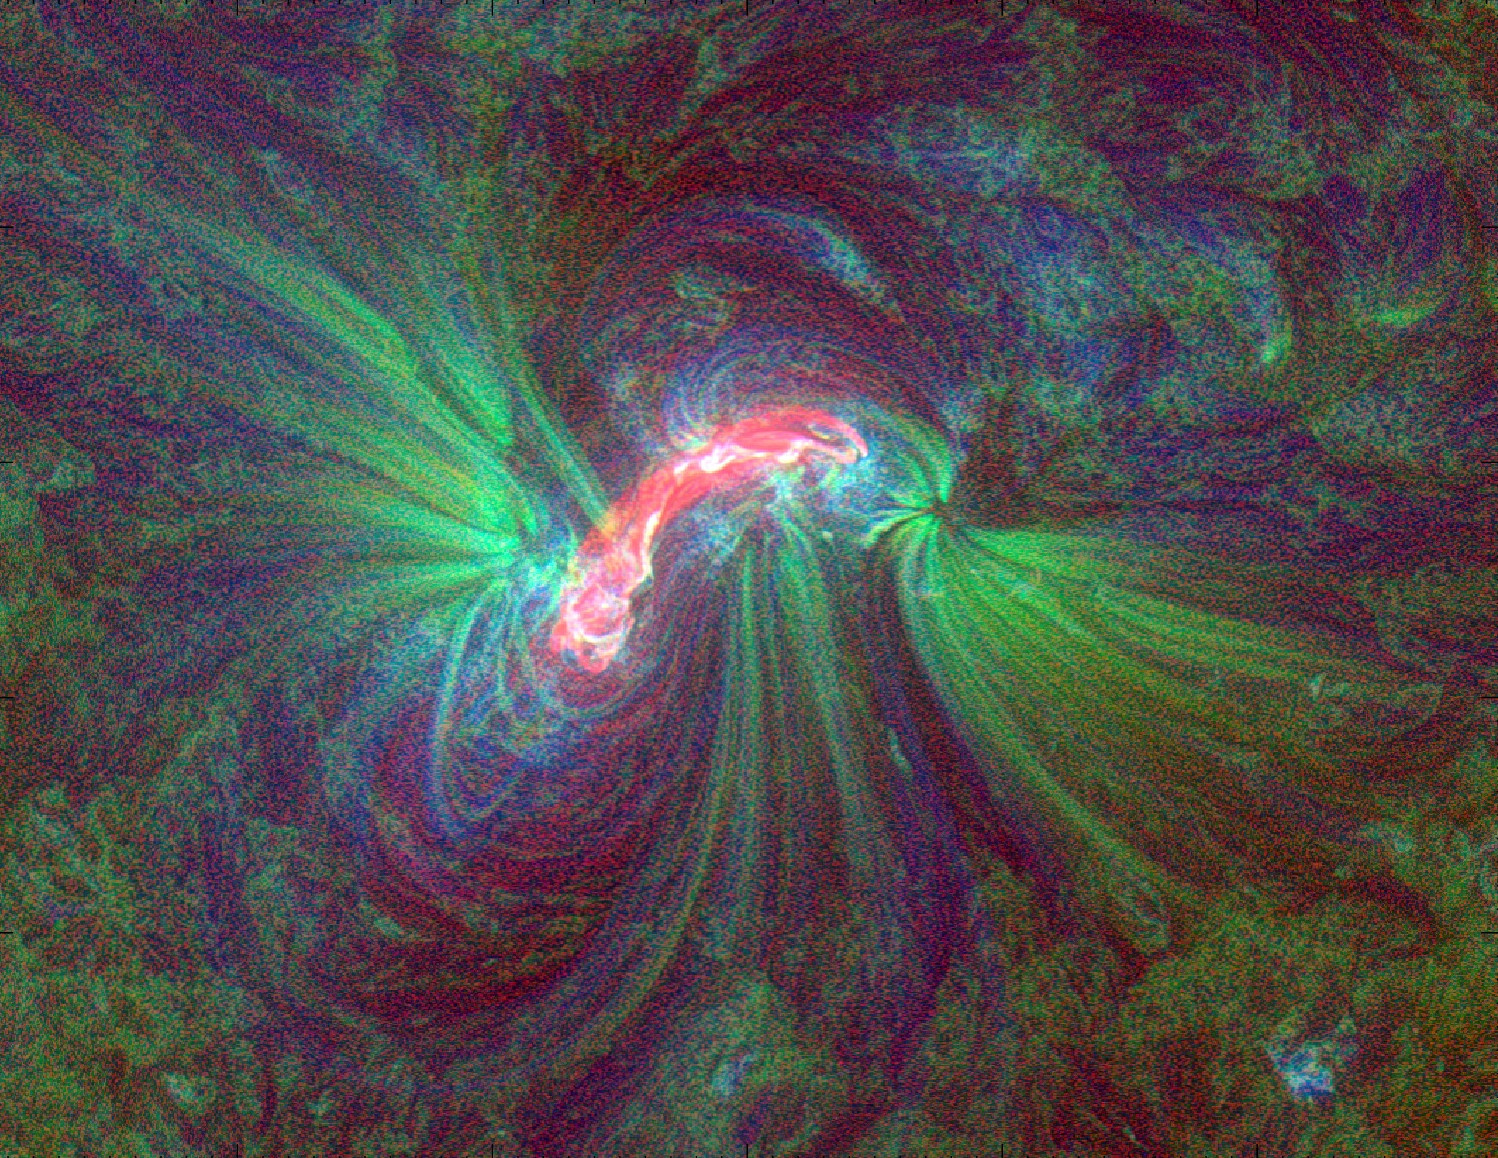
\includegraphics[width=\paperwidth]{figs/sigmoid_back.jpg}}
  \begin{frame}
    \titlepage
    \date{}
  \end{frame}
}
%%%%%%%%%%%%%%%%%%%%%%%%%%%%%%%%%%%%%%%%%%%%%%%%%%%%%%%%%%%%%%%%%%%%%%%%%%%%%%%%%%%%%%%%%%%%%%%%%%%

% im assuming this comes from the titles/frames i make later in 
\begin{frame}{Outline}
\tableofcontents
% \tableofcontents[hideallsubsections]
\end{frame}

%%%%%%%%%%%%%%%%%%%%%%%%%%%%%%%%%%%%%%%%%%%%%%%%%%%%%%%%%%%%%%%%%%%%%%%%%%%%%%%%%%%%%%%%%%%%%%%%%%%



%%%%%%%%%%%%%%%%%%%%%%%%%%%%%%%%%%%%%%%%%%%%%%%%%%%%%%%%%%%%%%%%%%%%%
%% Thermodynamics of a flare related on-disk active region sigmoid
%%%%%%%%%%%%%%%%%%%%%%%%%%%%%%%%%%%%%%%%%%%%%%%%%%%%%%%%%%%%%%%%%%%%

\begin{frame}{\normalsize Thermodynamics of a flare related
on-disk active region sigmoid}

\vspace{-10mm}
\tcbset{enhanced, attach boxed title to top center = {yshift = -3mm, yshifttext = -1mm}, colback = blue!5!white, colframe = blue!75!black, colbacktitle = red!80!black, fonttitle = \bfseries\small, boxed title style = {size = small, colframe = red!50!black}}

% Sigmoids
 \begin{tcolorbox}[title=Sigmoids, width=72mm, left=1mm, beforeafter skip=5mm, beforeafter = 10mm, right = 1mm]
\scriptsize  $\bullet$~Show S-shaped (reverse S or two J-shaped) structure \\
             $\bullet$~Highly sheared and twisted loops that are formed along
the polarity inversion line \\
             $\bullet$~Considered to be one of the best pre-eruption signatures
\end{tcolorbox}

%define research objectives
\begin{tcolorbox}[title=Research objective, width=72mm, left=1mm, beforeafter skip=1mm, beforeafter = 10mm, right = 1mm]
\scriptsize  $\bullet$~Investigation of temperature of a sigmoid during their
lifetime on solar disk \\
             $\bullet$~Relationship between sigmoids and solar flares \\
             $\bullet$~How temperature of a sigmoid varies during the
impulsive, peak and decay phase of flares
\end{tcolorbox}

% Adding two sigmoid images
\begin{textblock*}{30mm}(80mm,12mm)
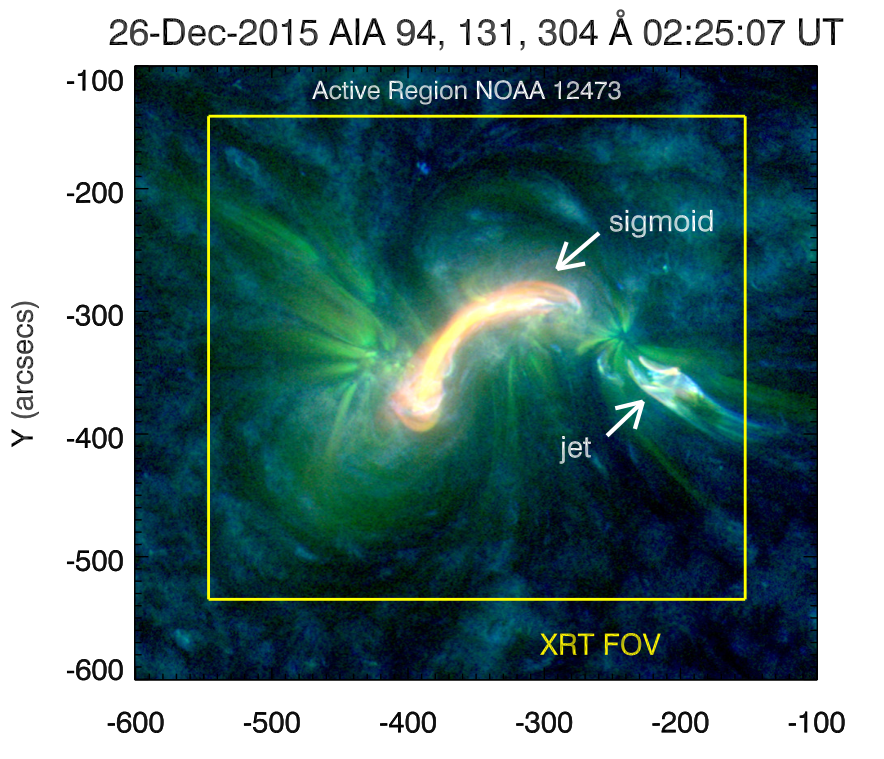
\includegraphics[height = 35mm, width=40mm]{figs/sigmoid_img}
\end{textblock*}
\begin{textblock*}{30mm}(83mm,50mm)
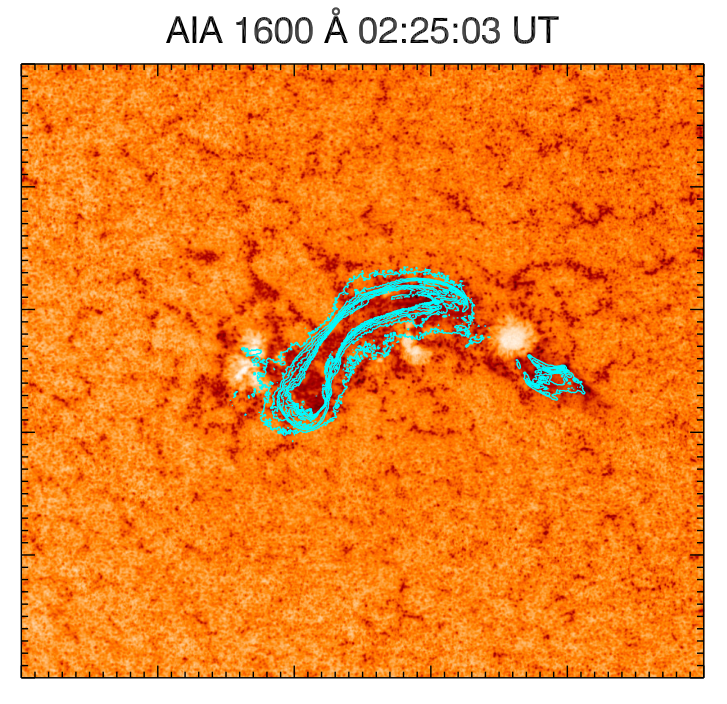
\includegraphics[height = 35mm, width=37mm]{figs/aia1600}
\end{textblock*}


% citation to paper
\begin{textblock*}{40mm}(83mm,88mm)
\tiny Mulay \textit{et al.} in preparation for MNRAS
 \end{textblock*}

\end{frame}

%%%%%%%%%%%%%%%%%%%%%%%%%%%%%%%%%%%%%%%%%%%%%%%%%%%%%%%%%%%%

\begin{frame}
 
 \vspace{-2mm}
 \begin{tcolorbox}[title = \bf Data collection, beforeafter skip=5mm, beforeafter = 10mm, right = 1mm,colframe=blue!50!black]
\scriptsize  $\bullet$~Using X-ray (Hinode/XRT) and EUV (SDO/AIA) imaging observations \\
             $\bullet$~Full disk XRT images from the Solar Monitor website, XRT event archive \\
             $\bullet$~On-disk sigmoids between $\pm$ 50$^{degree}$ longitude - 2010 – 2018 - $>$ 50 events
\end{tcolorbox}

\begin{tcolorbox}[title = \bf Methodology, beforeafter skip=5mm, beforeafter = 10mm, right = 1mm,colframe=blue!50!black]
\scriptsize  $\bullet$~Temperature analysis using different methods such as \\
             $\bullet$~\textcolor{red}{Filter ratio} -- two XRT channels, AIA 94 and 131~{\AA} channels,
GOES X-ray fluxes from two filters \\
             $\bullet$~\textcolor{red}{Emission measure analysis} using AIA observations -- Cheung et al. 2015 \\
             $\bullet$~Study of \textcolor{red}{Fe~{\sc xviii} emission from AIA 94~{\AA} channel} (Del Zanna 2013)
\end{tcolorbox}

\begin{tcolorbox}[title = \textbf{Sigmoid observation}, beforeafter skip=5mm, beforeafter = 10mm, right = 1mm,colframe=blue!50!black]
\scriptsize  $\bullet$~\textcolor{red}{Dec. 24 - 28, 2015} -- Sigmoid - NOAA AR 12473 - 4 B, 11 C and 2 M X-ray class \\
\scriptsize  $\bullet$~Dec. 26, 2015 -- C1.6 GOES flare - only brightening along sigmoid \\
\scriptsize  $\bullet$~Dec. 28, 2015 -- M1.8 GOES flare - sigmoid eruption \\
\end{tcolorbox}

\end{frame}
%%%%%%%%%%%%%%%%%%%%%%%%%%%%%%%%%%%%%%%%%%%%%%%%%%%%%%%%%%%%%%%%%%%%%%%%%%%%%%%


%%%%%%%%%%%%%%%%%%%%%%%%%%%%%%%%%%%%%%%%%%%%%%%%%%%%%%%%%%%%%%%%%%%%%%%%%%%%%%%%%%%%%%%%%%%%%%%%%%%


\begin{frame}{Introduction to Active Region Sigmoids}
\section{Sigmoids}
\begin{columns}[t]
\column{0.45\textwidth}
\begin{itemize}
 \item Active regions often show S-shaped structures in the corona
 \item highly sheared and twisted loops that are formed along the polarity inversion line
 \item considered to be one of the best pre-eruption
signatures
\end{itemize}

\column{0.45\textwidth}
\includemedia[
  activate=pageopen,
  width=100pt,height=100pt,
  addresource=exavimp4.mp4,
  flashvars={%
     source=exavimp4.mp4% same path as in addresource!
%      position = c
%   &autoPlay=true%    % optional configuration
   &loop=true%        % variables
  }  
]{}{media9/players/VPlayer.swf}
\end{columns}
\end{frame}
%%%%%%%%%%%%%%%%%%%%%%%%%%%%%%

\begin{frame}
 
 
 
 % Adding two sigmoid images
%  \vspace{-20mm}
% \begin{textblock*}{60mm}(1mm,1mm)
% \includegraphics[trim = 1 10 10 1, clip, width=1.2\linewidth]{figs/aia_context2}
% \end{textblock*}
% \begin{textblock*}{30mm}(83mm,50mm)
% \includegraphics[height = 35mm, width=37mm]{figs/aia_context2}
% \end{textblock*}
% 
% \tcbset{colframe=blue!50!black,colback=white,colupper=red!50!black, fonttitle=\bfseries,nobeforeafter,center title}
% \tcbox[tcbox raise base]{Sigmoid location in AIA, SOT and HMI images}

% citation to paper
\begin{textblock*}{80mm}(25mm,4mm)
\small \bf \textcolor{darkblue}{Sigmoid location in AIA, SOT and HMI images}
 \end{textblock*}

% Adding two sigmoid images
\begin{textblock*}{70mm}(20mm,10mm)
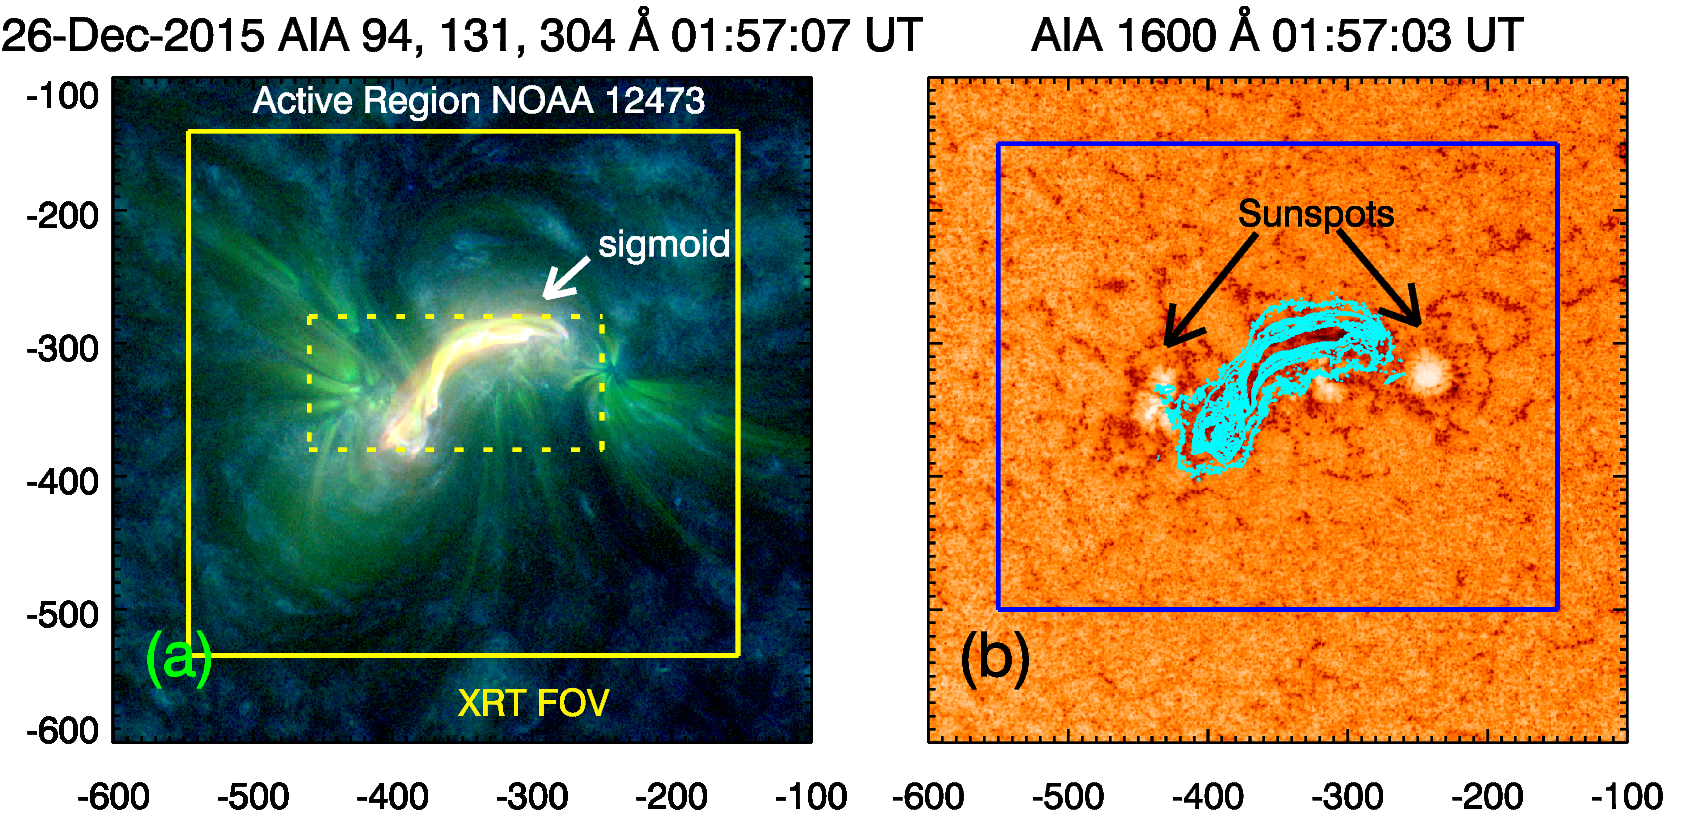
\includegraphics[height = 20mm, width = 40mm]{figs/sig1}
\end{textblock*}
\begin{textblock*}{70mm}(70mm,10mm)
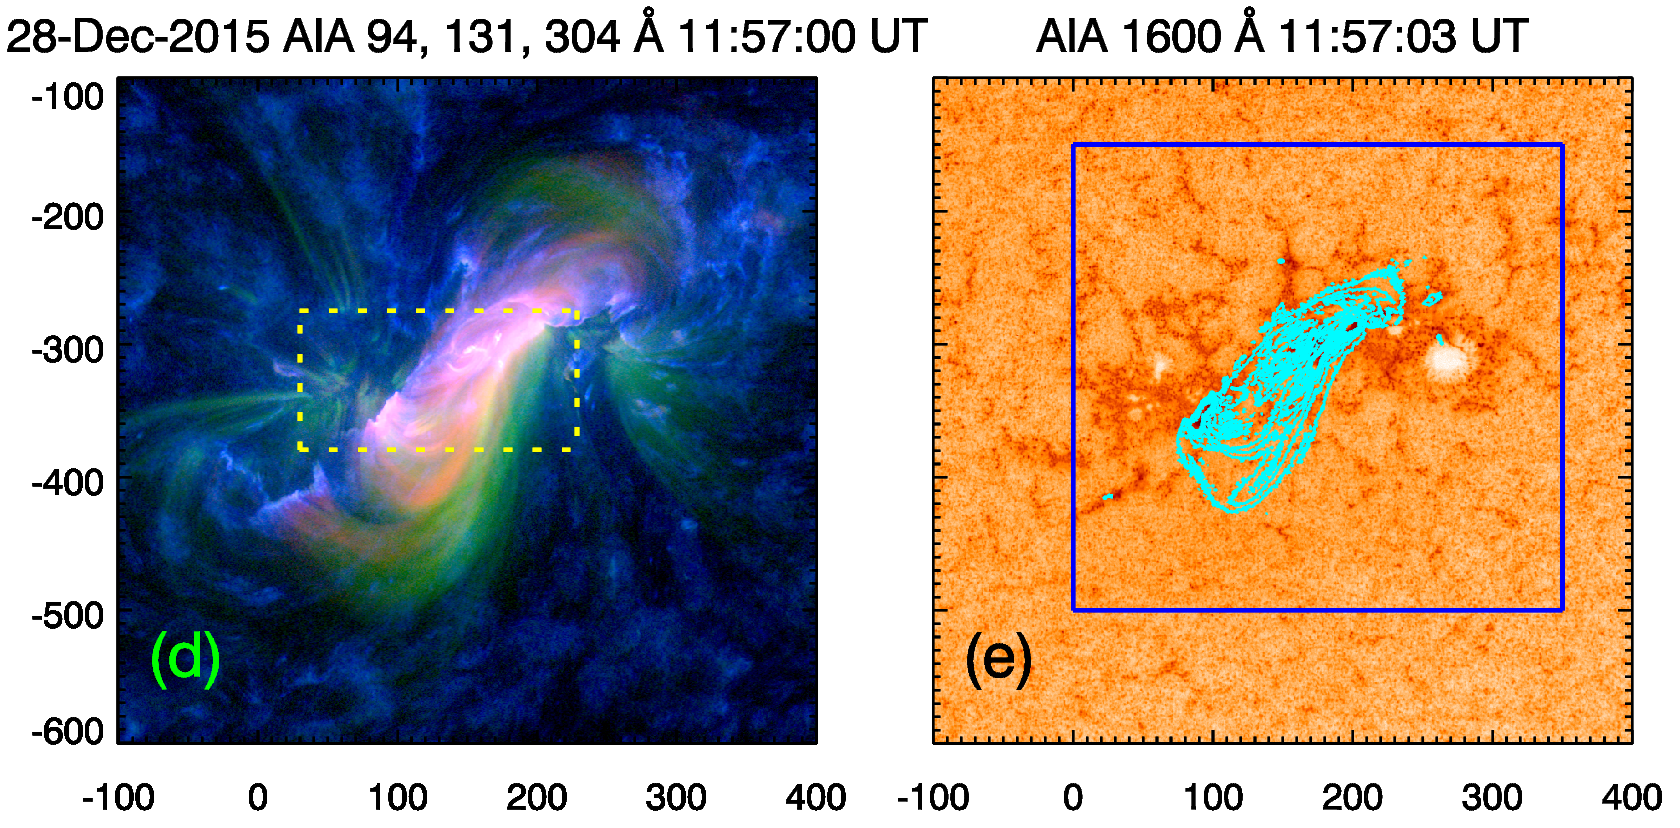
\includegraphics[height = 20mm, width = 40mm]{figs/sig2}
\end{textblock*}

% Adding two sigmoid images
\begin{textblock*}{200mm}(3mm,42mm)
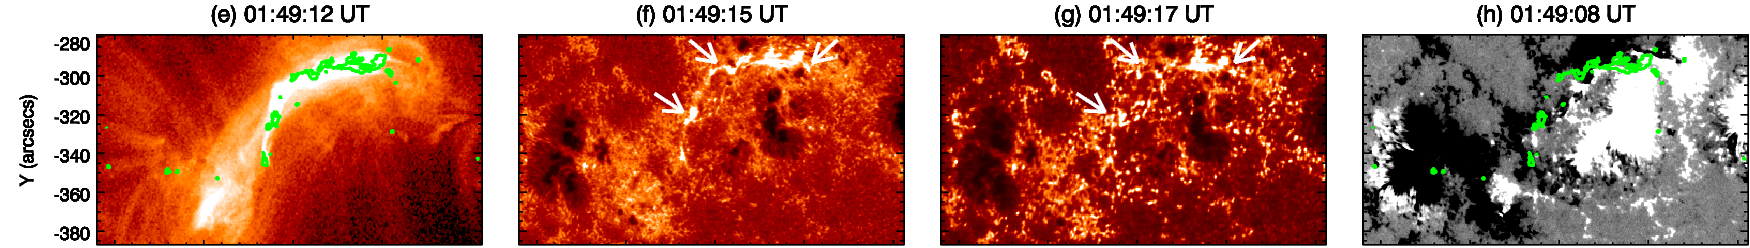
\includegraphics[height = 17mm, width = 120mm]{figs/sig3}
\end{textblock*}
\begin{textblock*}{200mm}(3mm,59mm)
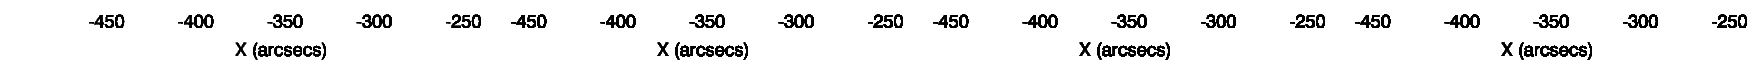
\includegraphics[height = 5mm, width = 120mm]{figs/sig4}
\end{textblock*} 

% Adding two sigmoid images
\begin{textblock*}{205mm}(4mm,65mm)
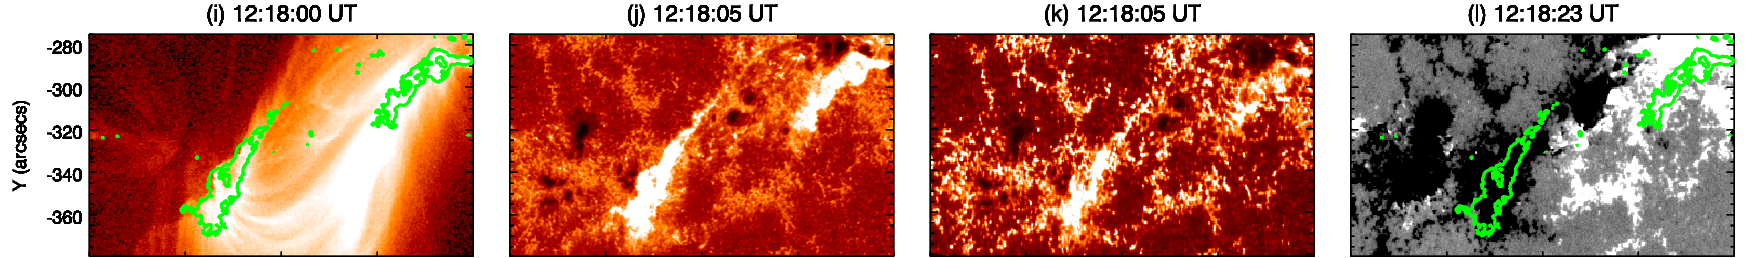
\includegraphics[height = 16mm, width = 120mm]{figs/sig5}
\end{textblock*}
\begin{textblock*}{210mm}(4mm,81.5mm)
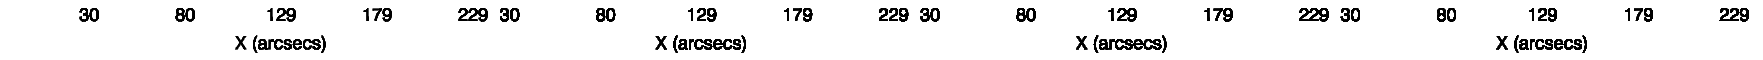
\includegraphics[height = 4mm, width = 121mm]{figs/sig6}
\end{textblock*} 
 
% Adding two sigmoid images
\begin{textblock*}{40mm}(16mm,35mm)
\scriptsize \textcolor{darkblue}{AIA 94~{\AA}}
\end{textblock*}
\begin{textblock*}{40mm}(40mm,35mm)
\scriptsize \textcolor{darkblue}{SOT Ca~{\sc ii} 3968~{\AA}}
\end{textblock*} 
  
% Adding two sigmoid images
\begin{textblock*}{40mm}(73mm,35mm)
\scriptsize \textcolor{darkblue}{AIA 1700~{\AA}}
\end{textblock*}
\begin{textblock*}{40mm}(97mm,35mm)
\scriptsize \textcolor{darkblue}{HMI LOS $\pm$ 100~G}
\end{textblock*} 
  
 
\end{frame}



%%%%%%%%%%%%%%%%%%%%%%%%%%%%%%


%%%%%%%%%%%%%%%%%%%%%%%%%%%%%%%%%%%%%%%%%%%
%% Adjust 2x2 or 3x3 figs in a frame
%%%%%%%%%%%%%%%%%%%%%%%%%%%%%%%%%%%%%%%%%%%
\begin{frame}{Adjust 1x2 or 1x3 figs in a frame}
\begin{figure}
  \centering
  \subfloat[First subfigure\label{fig:a}]{
\includegraphics[height=2cm,width=3cm]{figs/ORCIDiD_icon.png}}\qquad
  \subfloat[Second subfigure\label{fig:b}]{
\includegraphics[height=2cm,width=3cm]{figs/ORCIDiD_icon.png}}
\caption{A figure}
\label{fig:1}
\end{figure}
  
\begin{figure}
  \centering
  \subfloat[Third subfigure\label{fig:c}]{
\includegraphics[height=2cm,width=3cm]{figs/ORCIDiD_icon.png}}\qquad    
  \subfloat[Fourth subfigure\label{fig:d}]{
\includegraphics[height=2cm,width=3cm]{figs/ORCIDiD_icon.png}}%\qquad
  \subfloat[Fifth subfigure\label{fig:e}]{
\includegraphics[height=2cm,width=3cm]{figs/ORCIDiD_icon.png}}
  \caption{Another figure}
\label{fig:2}
\end{figure}
\end{frame}
%%%%%%%%%%%%%%%%%%%%%%%%%%%%%%%%%%%%%%%%%%%%%%%%%%%

%%%%%%%%%%%%%%%%%%%%%%%%%%%%%%%%%%%%%%%%%%%%%%%%%%%%%%%%%%
%%% 2X2 figs
%%%%%%%%%%%%%%%%%%%%%%%%%%%%%%%%%%%%%%%%%%%%%%%%%%%%%%%%%%

\begin{frame}{2X2 figs}
    \begin{columns}[t]
        \column{.5\textwidth}
        
\includegraphics[width=\columnwidth,height=3cm]{figs/ORCIDiD_icon.png}
        \captionof{figure}{foo}
        
\includegraphics[width=\columnwidth,height=3cm]{figs/ORCIDiD_icon.png}
        \captionof{figure}{bar}
        \column{.5\textwidth}
        
\includegraphics[width=\columnwidth,height=3cm]{figs/ORCIDiD_icon.png}
        \captionof{figure}{foo}
        
\includegraphics[width=\columnwidth,height=3cm]{figs/ORCIDiD_icon.png}
        \captionof{figure}{bar}
    \end{columns}
\end{frame}

%%%%%%%%%%%%%%%%%%%%%%%%%%%%%%%%%%%%%%%%%%%%%%%%%%%%%%%%%%%%%%

%%%%%%%%%%%%%%%%%%%%%%%%%%%%%%%%%%%%%%%%%%%%%%%%%%%%%%%%
%%% 3X2 figs
%%%%%%%%%%%%%%%%%%%%%%%%%%%%%%%%%%%%%%%%%%%%%%%%%%%%%%%%%%
\begin{frame}{2X3 figs}
    \begin{columns}[t]
        \column{.25\textwidth}
        
\includegraphics[width=\columnwidth,height=3cm]{figs/ORCIDiD_icon.png}
        \captionof{figure}{foo}
        
\includegraphics[width=\columnwidth,height=3cm]{figs/ORCIDiD_icon.png}
        \captionof{figure}{bar}
        \column{.25\textwidth}
        
\includegraphics[width=\columnwidth,height=3cm]{figs/ORCIDiD_icon.png}
        \captionof{figure}{foo}
        
\includegraphics[width=\columnwidth,height=3cm]{figs/ORCIDiD_icon.png}
        \captionof{figure}{bar}
        \column{.25\textwidth}
        
\includegraphics[width=\columnwidth,height=3cm]{figs/ORCIDiD_icon.png}
        \captionof{figure}{foo}
        
\includegraphics[width=\columnwidth,height=3cm]{figs/ORCIDiD_icon.png}
        \captionof{figure}{bar}
    \end{columns}
\end{frame}
%%%%%%%%%%%%%%%%%%%%%%%%%%%%%%%%%%%%%%%%%%%%%%%%%%%%%%%%%%%%%%

%%%%%%%%%%%%%%%%%%%%%%%%%%%%%%%%%%%%%%%%%%%%%%
%% Text in a Column + figs in a column
%%%%%%%%%%%%%%%%%%%%%%%%%%%%%%%%%%%%%%%%%%%%%%

\begin{frame}{Two columns - Text + figs}
    \begin{columns}[T, onlytextwidth]
        \begin{column}{0.5\textwidth}
            Some content here.\\
            Some content here.
            Some content here. 
        \end{column}
        \begin{column}{0.5\textwidth}
                \vskip-\baselineskip
            \begin{figure}
                \centering
                \begin{subfigure}%[t]{0.3 cm}
                    \left
                    
\includegraphics[height=1cm,width=2cm]{figs/ORCIDiD_icon.png}
                    \caption{Two line long caption}
                    \label{fig:sub1}
                \end{subfigure}\hskip 1em%
                \begin{subfigure}%[t]{0.3 cm}
                    \centering
                    
\includegraphics[height=1cm,width=2cm]{figs/ORCIDiD_icon.png}
                    \caption{One line caption}
                    \label{fig:sub2}
                \end{subfigure}
                \begin{subfigure}%[t]{0.3 cm}
                    \centering
                    
\includegraphics[height=1cm,width=2cm]{figs/ORCIDiD_icon.png}
                    \caption{One line caption}
                    \label{fig:sub1}
                \end{subfigure}\hskip 1em%
                \begin{subfigure}%[t]{0.3 cm}
                    \centering
                    
\includegraphics[height=1cm,width=2cm]{figs/ORCIDiD_icon.png}
                    \caption{Two line long caption}
                    \label{fig:sub2}
                \end{subfigure}
            \end{figure}
        \end{column}
    \end{columns}
\end{frame}
%%%%%%%%%%%%%%%%%%%%%%%%%%%%%%%%%%%%%%%

%%%%%%%%%%%%%%%%%%%%%%%%%%%%%%%%%%%%%%%%%%%%%%%%%%%
%%%%% Anumber of images
%%%%%%%%%%%%%%%%%%%%%%%%%%%%%%%%%%%%%%%%%%%%%%%%%%%

\begin{frame}
\begin{figure}[!htpb]
\label{fig:leslie}

\includegraphics[width=2.5cm]{figs/ORCIDiD_icon.png}

\includegraphics[width=2.5cm]{figs/ORCIDiD_icon.png}

\includegraphics[width=2.5cm]{figs/ORCIDiD_icon.png}

\includegraphics[width=2.5cm]{figs/ORCIDiD_icon.png}

\includegraphics[width=2.5cm]{figs/ORCIDiD_icon.png}

\includegraphics[width=2.5cm]{figs/ORCIDiD_icon.png}

\includegraphics[width=2.5cm]{figs/ORCIDiD_icon.png}

\includegraphics[width=2.5cm]{figs/ORCIDiD_icon.png}

\includegraphics[width=2.5cm]{figs/ORCIDiD_icon.png}

\includegraphics[width=2.5cm]{figs/ORCIDiD_icon.png}

\includegraphics[width=2.5cm]{figs/ORCIDiD_icon.png}

\caption{Leslie Lamport and his TeXbook.}
\end{figure}
\end{frame}
%%%%%%%%%%%%%%%%%%%%%%%%%%%%%%%%%%%%%%%%%%%%%%%%%%%%


%%%%%%%%%%%%%%%%%%%%%%%%%%%%%%%%%
%% Background image with text
%%%%%%%%%%%%%%%%%%%%%%%%%%%%%%%%%

{\usebackgroundtemplate{%
  
\includegraphics[width=\paperwidth,height=\paperheight]{figs/ORCIDiD_icon.png}} 
\begin{frame}{Background image with text}
 \color{yellow}{ABCD}
 \begin{textblock}{10.0}(1,2)
  \textcolor{yellow}{\textbf{This is the title of the presentation}}
 \end{textblock}
 

\end{frame}}
%%%%%%%%%%%%%%%%%%%%%%%%%%%%%%%%%%%%

%%%%%%%%%%%%%%%%%%%%%%%%%%%%%%%%%%%%%%%%%
%% Background image with text + block
%%%%%%%%%%%%%%%%%%%%%%%%%%%%%%%%%%%%%%%%%

{\usebackgroundtemplate{%
  
\includegraphics[width=\paperwidth,height=\paperheight]{figs/ORCIDiD_icon.png}} 
\begin{frame}{Background image with text}
\vspace{2em}
\begin{block}{Block Title}
Lorem ipsum dolor sit amet, consectetur adipisicing elit, 
sed do eiusmod tempor incididunt ut labore et 
dolore magna aliqua.
\end{block}
\end{frame}}

%%%%%%%%%%%%%%%%%%%%%%%%%%%%%%%%%
%% Background image with text
%%%%%%%%%%%%%%%%%%%%%%%%%%%%%%%%%

{\usebackgroundtemplate{%
  
\includegraphics[width=5 cm,height=5 cm]{figs/ORCIDiD_icon.png}} 
\begin{frame}
 \begin{textblock}{10.0}(1,2)
  \textcolor{red}{\textbf{This is the title of the presentation}}\\
  ABD
  
 \end{textblock}
\end{frame}}

%%%%%%%%%%%%%%%%%%%%%%%%%%%%%%%%%%%%


%%%%%%%%%%%%%%%%%%%%%%%%%%%%%%%%%
%% images with text
%%%%%%%%%%%%%%%%%%%%%%%%%%%%%%%%%
\begin{frame}{Positioning a single image}
 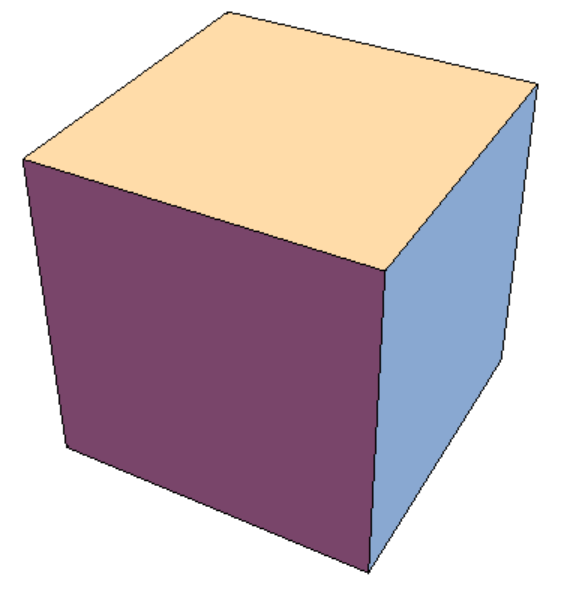
\includegraphics[width=3cm, heigth=3cm]{figs/cube}
 \setlength{\TPHorizModule}{\textwidth}
 \setlength{\TPVertModule}{\textwidth}
 \begin{textblock*}{200}(50,200)
  || Shree Swami Samartha||
 \end{textblock*}
 \begin{textblock*}{10pt}(100pt,150pt)
\small
\begin{equation*}
    \mathbf {H} = \frac{1}{2}\left( - \omega_{\mathrm{m}} + {\color{red}\delta \lambda(x)} \cos 2\theta_{\mathrm{m}} \right) \sigma_3 - \frac{  {\color{red}\delta \lambda(x)}  }{2} \sin \theta_{\mathrm{m}} \sigma_1
\end{equation*}
\end{textblock*}

\end{frame}

%%%%%%%%%%%%%%%%%%%%%

%%%%%%%%%%%%%%%%%%%%%%%%%%%%%%%%%%
%%% Different frame boxes
%%%%%%%%%%%%%%%%%%%%%%%%%%%%%%%%%%
\begin{frame}{Different types of boxes}

\framebox{This is a framebox}

\begin{shaded}
 This is a shaded text.
\end{shaded}

\shadowbox{This is a shadowbox.}

\doublebox{This is a doublebox.}

\ovalbox{This is a ovalbox.}

\begin{mdframed}[backgroundcolor = yellow]
This is an mdframed text with yellow Background. 
\end{mdframed}

\end{frame}
%%%%%%%%%%%%%%%%%%%%%%%%%%%%%%%%%%%%%%%%%

%%%%%%%%%%%%%%%%%%%%%%%%%%%%%%%%%%
%%% Different frame boxes
%%%%%%%%%%%%%%%%%%%%%%%%%%%%%%%%%%

\begin{frame}{Different types of boxes (cont.)}
\begin{shadowblock}
 This is a boxed environment with smein-transparent shadow.
\end{shadowblock}

\begin{tcolorbox}[enhanced,attach boxed title to top center={yshift=-3mm,yshifttext=-1mm},
  colback=blue!5!white,colframe=blue!75!black,colbacktitle=red!80!black,
  title=New title,fonttitle=\bfseries,
  boxed title style={size=small,colframe=red!50!black} ]
  This box uses a \textit{boxed title}. The box of the title can be formatted independently from the main box.
\end{tcolorbox}

\begin{tcolorbox}[enhanced,fit to height=5cm,
  colback=green!25!black!10!white,colframe=green!75!black,title=Fit box (5cm),
  drop fuzzy shadow,watermark color=white,watermark text=watermark test]
%   \lipsum[1-4]
    Hello Matthew
\end{tcolorbox}
\end{frame}
%%%%%%%%%%%%%%%%%%%%%%%%%%%%%%%%%%%%%%%%%%%%%

%%%%%%%%%%%%%%%%%%%%%%%%%%%%%
%%%% Arrows
%%%%%%%%%%%%%%%%%%%%%%%%%%%%

\begin{frame}
        \begin{itemize}
            \item This \MVRightarrow{} that
            \item This $\shortrightarrow$ that
            \item This \textrightarrow{} that
            \item This $\rightarrow$ that
            \item This $\longrightarrow$ that
        \end{itemize}
        
        \begin{itemize}
    \item This $\Rightarrow$ that
    \item This $\Longrightarrow$ that
    \item This $\implies$ that
\end{itemize}
    \end{frame}
    
%%%%%%%%%%%%%%%%%%%%%%%%%%%%%%%%%%%%%%%%%%    



%%%%%%%%%%%%%%%%%%%%%%%%%%%%%%%%%%%%%%%%%%%%%
%%%%%%% Arrow in equations pointing to text
%%%%%%% https://texample.net/tikz/examples/beamer-arrows/
%%%%%%% https://stuff.mit.edu/afs/athena/contrib/tex-contrib/beamer/pgf-1.01/doc/generic/pgf/version-for-tex4ht/en/pgfmanualse24.html
%%%%%%% https://tex.stackexchange.com/questions/9559/drawing-on-an-image-with-tikz/9562#9562
%%%%%%% https://tex.stackexchange.com/questions/459663/how-to-draw-arrows-from-floating-text-into-a-picture-in-beamer


%%%%%%%%%%%%%%%%%%%%%%%%%%%%%%%%%%%%%%%%%%%%%


% For every picture that defines or uses external nodes, you'll have to
% apply the 'remember picture' style. To avoid some typing, we'll apply
% the style to all pictures.
\tikzstyle{every picture}+=[remember picture]

% By default all math in TikZ nodes are set in inline mode. Change this to
% displaystyle so that we don't get small fractions.
\everymath{\displaystyle}

\begin{frame}
\frametitle{Rigid body dynamics}

\tikzstyle{na} = [baseline=-.5ex]

\begin{itemize}[<+-| alert@+>]
    \item Coriolis acceleration
        \tikz[na] \node[coordinate] (n1) {};
\end{itemize}

% Below we mix an ordinary equation with TikZ nodes. Note that we have to
% adjust the baseline of the nodes to get proper alignment with the rest of
% the equation.
\begin{equation*}
\vec{a}_p = \vec{a}_o+\frac{{}^bd^2}{dt^2}\vec{r} +
        \tikz[baseline]{
            \node[fill=blue!20,anchor=base] (t1)
            {$ 2\vec{\omega}_{ib}\times\frac{{}^bd}{dt}\vec{r}$};
        } +
        \tikz[baseline]{
            \node[fill=red!20, ellipse,anchor=base] (t2)
            {$\vec{\alpha}_{ib}\times\vec{r}$};
        } +
        \tikz[baseline]{
            \node[fill=green!20,anchor=base] (t3)
            {$\vec{\omega}_{ib}\times(\vec{\omega}_{ib}\times\vec{r})$};
        }
\end{equation*}

\begin{itemize}[<+-| alert@+>]
    \item Transversal acceleration
        \tikz[na]\node [coordinate] (n2) {};
    \item Centripetal acceleration
        \tikz[na]\node [coordinate] (n3) {};
\end{itemize}

% Now it's time to draw some edges between the global nodes. Note that we
% have to apply the 'overlay' style.
\begin{tikzpicture}[overlay]
        \path[->]<1-> (n1) edge [bend left] (t1);
        \path[->]<2-> (n2) edge [bend right] (t2);
        \path[->]<3-> (n3) edge [out=0, in=-90] (t3);
\end{tikzpicture}
\end{frame}

%%%%%%%%%%%%%%%%%%%%%%%%%%%%%%%%%%%%%%%%%%%%%%%%%%
%%% Draw a pie chart 
%%%%%%%%%%%%%%%%%%%%%%%%%%%%%%%%%%%%%%%%%%%%%%%%%%

\begin{frame}
\centering
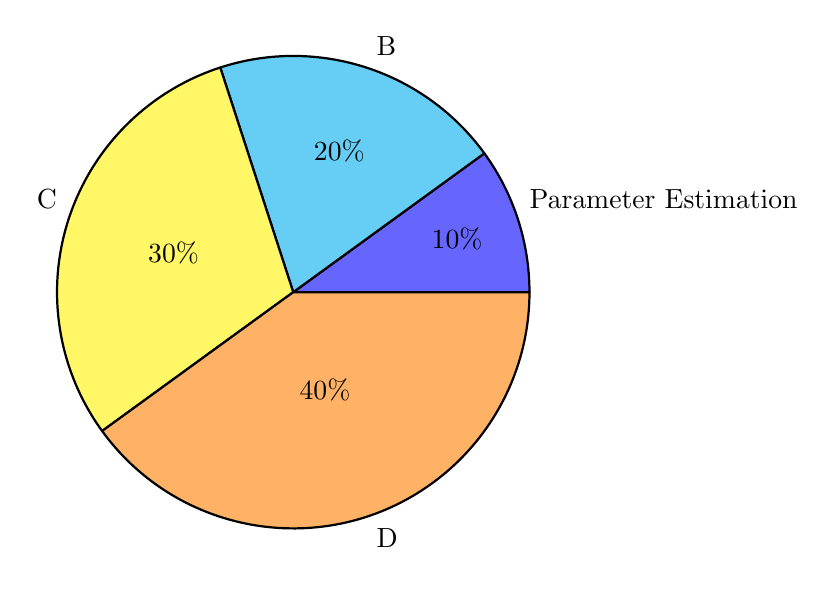
\begin{tikzpicture}
\pie{10/Parameter Estimation, 20/B, 30/C, 40/D}
\end{tikzpicture}
\end{frame}

\begin{frame}
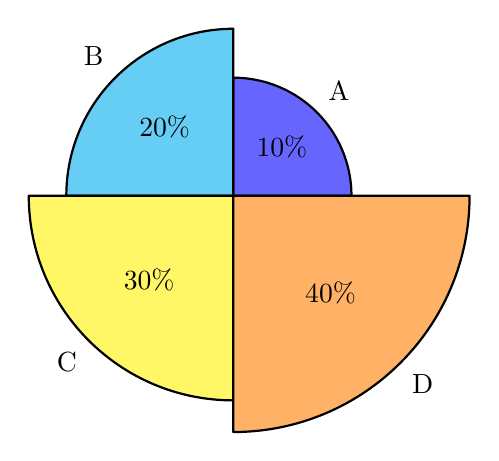
\begin{tikzpicture}
  \pie[polar]{10/A, 20/B, 30/C, 40/D}
\end{tikzpicture}
\end{frame}

\begin{frame}
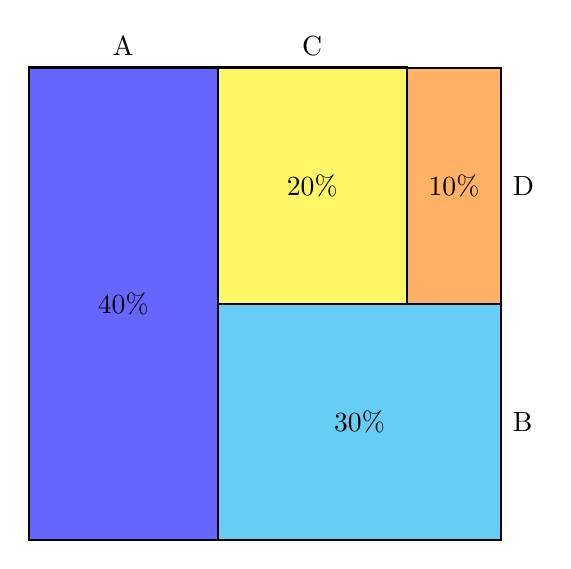
\begin{tikzpicture}
  \pie[square]{40/A, 30/B, 20/C, 10/D}
\end{tikzpicture}
\end{frame}

\begin{frame}
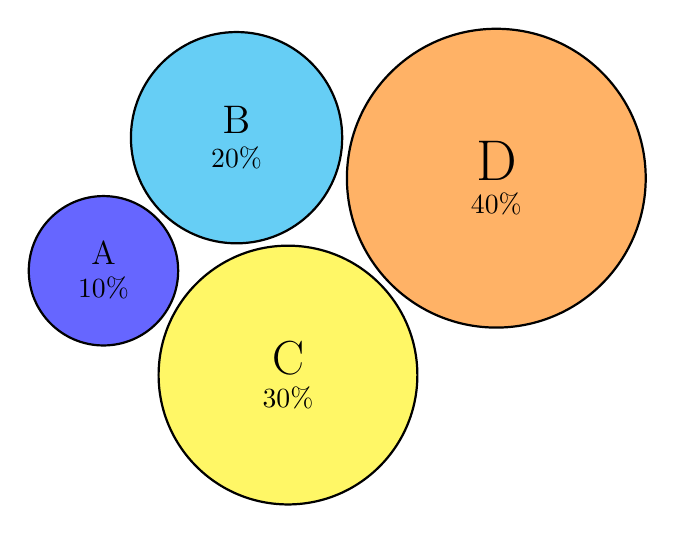
\begin{tikzpicture}
  \pie[cloud, text=inside, scale font]{10/A, 20/B, 30/C, 40/D}
\end{tikzpicture}
\end{frame}

%%%%%%%%%%%%%%%%%%%%%%%%%%%%%%%%%%%%%%%%%%%%%%%%%%%%%%%


\subsection[Themes]{Themes, colors and fonts}

\begin{frame}{Themes, colors and fonts}
\begin{itemize}
	\item 
		Themes can be changed with the command \cm{usetheme}. \pause 
		A list of the different themes can be found \wl{here}{http://deic.uab.es/~iblanes/beamer_gallery/index_by_theme.html}. \pause
	\item 
		The colors of a theme can be changed with the command \cm{usecolortheme}. \pause
		A list of the different colors can be found \wl{here}{http://deic.uab.es/~iblanes/beamer_gallery/index_by_color.html}. \pause
	\item 
		The fonts can be changed with the command \cm{usefonttheme}. \pause
		A list of the different fonts can be found here \wl{here}{http://deic.uab.es/~iblanes/beamer_gallery/index_by_font.html}. \pause
\end{itemize}
\textcolor{black}{See the difference in this equation}
\begin{equation}
	f(x) = x^{2345}\sin(x) .
\end{equation}
\end{frame}


\begin{frame}{Custom colors}
You can also define your own colors with the commands \cm{definecolor} and \cm{setbeamercolor}.
\end{frame}

%%%%%%%%%%%%%%%%%%%%%%%%%%%%%%%%%%%%%%%%%%%%%%%%%%%%%%%%%%%%%%%%%%%%%%%%%%%%%%%%%%%%%%%%%%%%%%%%%%%


\subsection[Frame numbers]{Frame numeration and foot}

\begin{frame}{Frame number}
The frame number can be added to the bottom of the slide with the command \cm{setbeamertemplate\{footline\}[frame number]}.
\end{frame}


\begin{frame}{Foot}
Alternative the foot of the presentation can be changed with further options for \cm{setbeamertemplate\{footline\}}.
\end{frame}

%%%%%%%%%%%%%%%%%%%%%%%%%%%%%%%%%%%%%%%%%%%%%%%%%%%%%%%%%%%%%%%%%%%%%%%%%%%%%%%%%%%%%%%%%%%%%%%%%%%

\subsection[Aspect]{Aspect ratio}

\begin{frame}{Aspect ratio}
With \cm{documentclass[aspectratio=169]\{beamer\}} you will create slides in 16:9 format.
\end{frame}

%%%%%%%%%%%%%%%%%%%%%%%%%%%%%%%%%%%%%%%%%%%%%%%%%%%%%%%%%%%%%%%%%%%%%%%%%%%%%%%%%%%%%%%%%%%%%%%%%%%
%%%%%%%%%%%%%%%%%%%%%%%%%%%%%%%%%%%%%%%%%%%%%%%%%%%%%%%%%%%%%%%%%%%%%%%%%%%%%%%%%%%%%%%%%%%%%%%%%%%

%%%%%%%%%%%%%%%%%%%%%%%%%%%%%%%%%%%%%%%%%%%%%%%%%%%%%%%%%%%%%%%%%%%%%%%%%%%%%%%%%%%%%%%%%%%%%%%%%%%

\subsection{Highlight current section}
% \tableofcontents[currentsubsection]
\begin{frame}{Where are we?}
Although most of the themes have a sidebar with the sections of the presentation, it is still for some people very useful to highlight the upcoming section and its contents. \pause
This can be achieved using the command \cm{tableofcontents[currentsection]} just after the section definition.
\end{frame}

%%%%%%%%%%%%%%%%%%%%%%%%%%%%%%%%%%%%%%%%%%%%%%%%%%%%%%%%%%%%%%%%%%%%%%%%%%%%%%%%%%%%%%%%%%%%%%%%%%%

\subsection{Columns}
\begin{frame}{Columns}
Columns can be used in order to separate content. \\[1cm]
\begin{columns}[t]
\column{0.45\textwidth}
	Some text in the first column. It is important to see here that the content in the columns are aligned to the top. You can choose t,c or b.
\column{0.45\textwidth}
	Some text the second column.
\end{columns}
\end{frame}

%%%%%%%%%%%%%%%%%%%%%%%%%%%%%%%%%%%%%%%%%%%%%%%%%%%%%%%%%%%%%%%%%%%%%%%%%%%%%%%%%%%%%%%%%%%%%%%%%%%

\subsection{Images, videos and attachments}
\begin{frame}{Embedding images}
You may want to use different kind of images like PNG and EPS figs. In order to be able to work with EPS figs you need to adapt your compilation procedure. Here you can see a PNG figure.
\begin{center}
	\includegraphics[width=0.2\textwidth]{figs/cube}
\end{center}
For conversion of PNG figs into EPS search in Google for a converter or go \wl{here}{http://www.tlhiv.org/rast2vec/}.
\end{frame}


\begin{frame}{Setting a link to a video}
You are also able to link videos to the created PDF using the command \cm{movie}.
\begin{center}
% 	\movie[externalviewer]{\includegraphics[width=3cm]{figs/arrow}}{videos/aia_xrt_simul_spire.mp4}
	\qquad
	\movie[externalviewer]{\includegraphics[width=2cm]{figs/cube}}{videos/exavi.avi} \\[0.3cm]
	\movie[externalviewer]{\includegraphics[width=3cm]{figs/arrow}}{videos/exmp4.mp4}
	\qquad
	\movie[externalviewer]{\includegraphics[width=2cm]{figs/cube}}{videos/exavimp4.mp4}
\end{center}
A fantastic explanation on how to convert videos with the completely free VLC player can be found \wl{here}{http://www.tweakandtrick.com/2014/01/convert-videos-vlc.html}.
\end{frame}


\begin{frame}{Other attachments}
You might also want to show other attached files, e.g., \att{manipulate}{run:attachments/manipulate.nb}.
\end{frame}

%%%%%%%%%%%%%%%%%%%%%%%%%%%%%%%%%%%%%%%%%%%%%%%%%%%%%%%%%%%%%%%%%%%%%%%%%%%%%%%%%%%%%%%%%%%%%%%%%%%

\subsection{Overlays: pause, visible, unconver, only}
\begin{frame}{Overlays: pause}
An itemized or enumerated list can be paused at several parts using the command \cm{pause}, e.g.
\begin{itemize}
	\pause
	\item first
	\pause
	\item second
	\pause
	\item third
	\item fourth
\end{itemize}
\end{frame}

\begin{frame}{Overlays: visible, unconver and only}
If a more elaborated form has to be presented, use unconver and only. Example: \\[0.3cm]

\begin{columns}[t]
\column{0.45\textwidth}
	Description of some concept \\
	\visible<2->{
	\begin{enumerate}
	\item	
		Point 1
	\visible<3->{
	\item
		Point 2
	\item
		Point 3
	\visible<5->{
	\item
		Point 4
	}
	}
	\end{enumerate}	
	}
\column{0.5\textwidth}
	\mbox{} \\
	\begin{overlayarea}{\textwidth}{0.4\textheight}
	\only<4-5>{\includegraphics[width=0.4\textwidth]{figs/cube}}
	\only<6->{\includegraphics[width=0.9\textwidth]{figs/arrow}}
	\end{overlayarea}
	More Text.
\end{columns}

\end{frame}

%%%%%%%%%%%%%%%%%%%%%%%%%%%%%%%%%%%%%%%%%%%%%%%%%%%%%%%%%%%%%%%%%%%%%%%%%%%%%%%%%%%%%%%%%%%%%%%%%%%

\subsection{Tables}
\begin{frame}{Presentation of data}
As in the other \LaTeX{} documents you can also use here tables in order to present data.
\begin{center}
	\begin{tabular}{l|ccr}
	\hline\hline	
	 & bla & ble & bli \\ \hline
	first
		& sdfajfdlkö
		& sdjdklf
		& djk \\
	second
		& sfd
		& fdgdfgds
		& dfgshgsdfh \\ \hline\hline
	\end{tabular}
\end{center}
\end{frame}

%%%%%%%%%%%%%%%%%%%%%%%%%%%%%%%%%%%%%%%%%%%%%%%%%%%%%%%%%%%%%%%%%%%%%%%%%%%%%%%%%%%%%%%%%%%%%%%%%%%

\subsection[Blocks]{Text blocks, definitions, theorems and proofs}

\begin{frame}{Text blocks}
You have the possibility to use the environment \cm{block} for separating important content and concepts from the rest of the text. \pause
\begin{block}{Title of the concept}
	Description of the concept comes in this region. You are able to define more stuff in this region, e.g. equations
	\begin{equation}
		a + b = c
	\end{equation}
	and more.
\end{block}
\end{frame}

\begin{frame}{Text blocks}
More blocks \pause
\begin{definition}[Name]
	Description
\end{definition}
\pause
\begin{theorem}[Name]
	Description
\end{theorem}
\pause
\begin{proof}
	Proof
\end{proof}
\end{frame}

%%%%%%%%%%%%%%%%%%%%%%%%%%%%%%%%%%%%%%%%%%%%%%%%%%%%%%%%%%%%%%%%%%%%%%%%%%%%%%%%%%%%%%%%%%%%%%%%%%%

\subsection[Math]{Mathematical content}
\begin{frame}{Mathematical content}
Of course you are able to create also equations
\begin{equation}
	m \ddot{x} = \sum_{i=1}^n F_i \quad , \quad
	\delta H = 0 \quad , \quad
	x(t) = \int_0^t\limits{ v(s) }ds
\end{equation}
separately or in the text $f(x)=x^2$ using the common commands.
\end{frame}

%%%%%%%%%%%%%%%%%%%%%%%%%%%%%%%%%%%%%%%%%%%%%%%%%%%%%%%%%%%%%%%%%%%%%%%%%%%%%%%%%%%%%%%%%%%%%%%%%%%
%%%%%%%%%%%%%%%%%%%%%%%%%%%%%%%%%%%%%%%%%%%%%%%%%%%%%%%%%%%%%%%%%%%%%%%%%%%%%%%%%%%%%%%%%%%%%%%%%%%

\section[Handout]{Presentation handout}

\begin{frame}{Table of contents}
\tableofcontents[currentsection,hidesubsections]
\end{frame}

%%%%%%%%%%%%%%%%%%%%%%%%%%%%%%%%%%%%%%%%%%%%%%%%%%%%%%%%%%%%%%%%%%%%%%%%%%%%%%%%%%%%%%%%%%%%%%%%%%%

\subsection{Handout option}
\begin{frame}{How to create a handout?}
As you could see using the command pause a lot of PDF pages are created. May be you will want to give an handout of your presentation without the pauses. This can be done with the document class option \cm{handout}. This will then ignore all pauses and a "reduced" PDF will be created.
\end{frame}

%%%%%%%%%%%%%%%%%%%%%%%%%%%%%%%%%%%%%%%%%%%%%%%%%%%%%%%%%%%%%%%%%%%%%%%%%%%%%%%%%%%%%%%%%%%%%%%%%%%

\begin{frame}
 
 \begin{thebibliography}{10}
\bibitem{Goldbach1742}[Goldbach, 1742]
Christian Goldbach.
\newblock A problem we should try to solve before the ISPN ’43 deadline,
\newblock \emph{Letter to Leonhard Euler}, 1742.
\end{thebibliography}
and he can then add a citation:
\begin{block}{Open Questions}
Is every even number the sum of two primes?
\cite{Goldbach1742}
\end{block}
\end{frame}


%%%%%%%%%%%%%%%%%%%%%%%%%%%%%%%%%%%%%%%%%%%%%%%%%%%%%%%%%%%%%%%%%%%%%%%%%%%%%%%%%%%%%%%%%%%%%%%%%%%

% %%%%%%%%%%%%%%%%%%%%%%%%%%%%%%%%%%%%%%%%%%%%%%%%%%%%%%%
% \begin{frame}{Tiral}
% 
% 
%  \begin{tcolorbox}[enhanced,attach boxed title to top center={yshift=-3mm,yshifttext=-1mm},
%   colback=blue!5!white,colframe=blue!75!black,colbacktitle=red!80!black,
%   title=Research objective,fonttitle=\bfseries,width=(\linewidth-10mm)/2, 
%   boxed title style={size=small,colframe=red!50!black} ]
% %        \hspace{-pt}
% 1) ABC
% 
%   \begin{itemize}
%      \item \small S-shaped topology in the core of active region
%      \item \small Twisted and sheared structure observed \\
%      prior to CME eruption
%     \end{itemize}
% \end{tcolorbox}
% \begin{tcolorbox}
%  XYC
% \end{tcolorbox}
% 
% 
% \tcbset{colback=red!5!white,fonttitle=\bfseries,width=(\linewidth-20mm)/2}
% \begin{tcolorbox}[enhanced,title=My title,
% frame style={left color=red!75!black,
% right color=blue!75!black}]
% \footnotesize Investigation of temperature during the impulsive, \\
% peak and decay phase of flares which are \\
% associated with eruptive and \\
% non-eruptive sigmoids
% \tcblower
% This is the lower part.
% \end{tcolorbox}
% \begin{tcolorbox}
%  ABC
% \end{tcolorbox}
% 
% 
%   
%   \vspace*{-3.5cm} \hspace*{8.9cm}\includegraphics[width=0.25\linewidth]{figs/sigmoid_img}
% %  \vspace*{-10pt} \hspace*{250pt}\includegraphics[width=0.25\linewidth]{figs/sigmoid_img}
%  \setlength{\TPHorizModule}{\textwidth}
%  \setlength{\TPVertModule}{\textwidth}
%  
% %  \begin{textblock*}{20}(200,50)
% %   includegraphics[width=0.5\linewidth]{figs/sigmoid_img}
% %  \end{textblock*}
%  
% %  \begin{textblock*}{200}(50,200)
% %   || Shree Swami Samartha||
% %  \end{textblock*}
% 
% %  \begin{textblock*}{10pt}(100pt,150pt)
% % \small
% % \begin{equation*}
% %     \mathbf {H} = \frac{1}{2}\left( - \omega_{\mathrm{m}} + {\color{red}\delta \lambda(x)} \cos 2\theta_{\mathrm{m}} \right) \sigma_3 - \frac{  {\color{red}\delta \lambda(x)}  }{2} \sin \theta_{\mathrm{m}} \sigma_1
% % \end{equation*}
% % \end{textblock*}
% 
% \end{frame}
% 
% %%%%%%%%%%%%%%%%%%%%%
% 
% 
% %%%%%%%%%%%%%%%%%%%%%%%%%%%%%%
% %%% {Tasks with pauses}
% %%%%%%%%%%%%%%%%%%%%%%%%%%%%%%
% 
% \begin{frame}{Tasks with pauses}
% Text always present
% 
% \begin{itemize}
% \item<2-> Item 1
% 
% \item<3-> Item 2
% 
% \item<4-> Item 3
% 
% \item<5-> Item 4
% \end{itemize}
% 
% \alt<4>{
% \begin{block}{Block to item 3}
% block 1
% \end{block}
% }
% {\visible<5>{
% \begin{block}{Block to item 4}
% block 2
% \end{block}
% }}
% \end{frame}
% %%%%%%%%%%%%%%%%%%%%%%%%%%%%%%%%%%%%%%%%%%%%%%%%%%%%%%%%
% %%%
% 
% %%%%%%%%%%%%%%%%%%%%%%%%%%%%%%%%%%%%%%%%%%%%%%%%%%%%%%%%%%%%%
% %%%% Images with pauses
% %%%%%%%%%%%%%%%%%%%%%%%%%%%%%%%%%%%%%%%%%%%%%%%%%%%%%%%%%%%%%%%%
% \begin{frame}{Images with pauses}
%   \frametitle{Images with pauses}
%   \begin{overlayarea}{\textwidth}{\textheight}
%     \begin{figure}
%       \centering
%       \only<1>
%         {%
%           \includegraphics[width=.4\textwidth]{figs/cube.PNG}%
%         }%
%       \only<2>
%         {%
%           \includegraphics[width=.4\textwidth]{figs/ORCIDiD_icon.png}%
%         }%
%       \only<3>
%         {%
%           \includegraphics[width=.4\textwidth]{figs/arrow.PNG}%
%         }%
%     \end{figure}
%   \end{overlayarea}      
% \end{frame}
% %%%%%%%%%%%%%%%%%%%%%%%%%%%%%%%%%%%%%%%%%%%%%%%%%%%%%%%%%
% 
% 
% %%%%%%%%%%%%%%%%%%%%%%%%%%%%%%%%%%%%%%%%%%%
% %% Adjust 2x2 or 3x3 figs in a frame
% %%%%%%%%%%%%%%%%%%%%%%%%%%%%%%%%%%%%%%%%%%%
% \begin{frame}{Adjust 1x2 or 1x3 figs in a frame}
% \begin{figure}
%   \centering
%   \subfloat[First subfigure\label{fig:a}]{\includegraphics[height=2cm,width=3cm]{figs/ORCIDiD_icon.png}}\qquad
%   \subfloat[Second subfigure\label{fig:b}]{\includegraphics[height=2cm,width=3cm]{figs/ORCIDiD_icon.png}}
% \caption{A figure}
% \label{fig:1}
% \end{figure}
%   
% \begin{figure}
%   \centering
%   \subfloat[Third subfigure\label{fig:c}]{\includegraphics[height=2cm,width=3cm]{figs/ORCIDiD_icon.png}}\qquad    
%   \subfloat[Fourth subfigure\label{fig:d}]{\includegraphics[height=2cm,width=3cm]{figs/ORCIDiD_icon.png}}%\qquad
%   \subfloat[Fifth subfigure\label{fig:e}]{\includegraphics[height=2cm,width=3cm]{figs/ORCIDiD_icon.png}}
%   \caption{Another figure}
% \label{fig:2}
% \end{figure}
% \end{frame}
% %%%%%%%%%%%%%%%%%%%%%%%%%%%%%%%%%%%%%%%%%%%%%%%%%%%
% 
% %%%%%%%%%%%%%%%%%%%%%%%%%%%%%%%%%%%%%%%%%%%%%%%%%%%%%%%%%%
% %%% 2X2 figs
% %%%%%%%%%%%%%%%%%%%%%%%%%%%%%%%%%%%%%%%%%%%%%%%%%%%%%%%%%%
% 
% \begin{frame}{2X2 figs}
%     \begin{columns}[t]
%         \column{.5\textwidth}
%         \includegraphics[width=\columnwidth,height=3cm]{figs/ORCIDiD_icon.png}
%         \captionof{figure}{foo}
%         \includegraphics[width=\columnwidth,height=3cm]{figs/ORCIDiD_icon.png}
%         \captionof{figure}{bar}
%         \column{.5\textwidth}
%         \includegraphics[width=\columnwidth,height=3cm]{figs/ORCIDiD_icon.png}
%         \captionof{figure}{foo}
%         \includegraphics[width=\columnwidth,height=3cm]{figs/ORCIDiD_icon.png}
%         \captionof{figure}{bar}
%     \end{columns}
% \end{frame}
% 
% %%%%%%%%%%%%%%%%%%%%%%%%%%%%%%%%%%%%%%%%%%%%%%%%%%%%%%%%%%%%%%
% 
% %%%%%%%%%%%%%%%%%%%%%%%%%%%%%%%%%%%%%%%%%%%%%%%%%%%%%%%%
% %%% 3X2 figs
% %%%%%%%%%%%%%%%%%%%%%%%%%%%%%%%%%%%%%%%%%%%%%%%%%%%%%%%%%%
% \begin{frame}{2X3 figs}
%     \begin{columns}[t]
%         \column{.25\textwidth}
%         \includegraphics[width=\columnwidth,height=3cm]{figs/ORCIDiD_icon.png}
%         \captionof{figure}{foo}
%         \includegraphics[width=\columnwidth,height=3cm]{figs/ORCIDiD_icon.png}
%         \captionof{figure}{bar}
%         \column{.25\textwidth}
%         \includegraphics[width=\columnwidth,height=3cm]{figs/ORCIDiD_icon.png}
%         \captionof{figure}{foo}
%         \includegraphics[width=\columnwidth,height=3cm]{figs/ORCIDiD_icon.png}
%         \captionof{figure}{bar}
%         \column{.25\textwidth}
%         \includegraphics[width=\columnwidth,height=3cm]{figs/ORCIDiD_icon.png}
%         \captionof{figure}{foo}
%         \includegraphics[width=\columnwidth,height=3cm]{figs/ORCIDiD_icon.png}
%         \captionof{figure}{bar}
%     \end{columns}
% \end{frame}
% %%%%%%%%%%%%%%%%%%%%%%%%%%%%%%%%%%%%%%%%%%%%%%%%%%%%%%%%%%%%%%
% 
% %%%%%%%%%%%%%%%%%%%%%%%%%%%%%%%%%%%%%%%%%%%%%%
% %% Text in a Column + figs in a column
% %%%%%%%%%%%%%%%%%%%%%%%%%%%%%%%%%%%%%%%%%%%%%%
% 
% \begin{frame}{Two columns - Text + figs}
%     \begin{columns}[T, onlytextwidth]
%         \begin{column}{0.5\textwidth}
%             Some content here.\\
%             Some content here.
%             Some content here. 
%         \end{column}
%         \begin{column}{0.5\textwidth}
%                 \vskip-\baselineskip
%             \begin{figure}
%                 \centering
%                 \begin{subfigure}%[t]{0.3 cm}
%                     \left
%                     \includegraphics[height=1cm,width=2cm]{figs/ORCIDiD_icon.png}
%                     \caption{Two line long caption}
%                     \label{fig:sub1}
%                 \end{subfigure}\hskip 1em%
%                 \begin{subfigure}%[t]{0.3 cm}
%                     \centering
%                     \includegraphics[height=1cm,width=2cm]{figs/ORCIDiD_icon.png}
%                     \caption{One line caption}
%                     \label{fig:sub2}
%                 \end{subfigure}
%                 \begin{subfigure}%[t]{0.3 cm}
%                     \centering
%                     \includegraphics[height=1cm,width=2cm]{figs/ORCIDiD_icon.png}
%                     \caption{One line caption}
%                     \label{fig:sub1}
%                 \end{subfigure}\hskip 1em%
%                 \begin{subfigure}%[t]{0.3 cm}
%                     \centering
%                     \includegraphics[height=1cm,width=2cm]{figs/ORCIDiD_icon.png}
%                     \caption{Two line long caption}
%                     \label{fig:sub2}
%                 \end{subfigure}
%             \end{figure}
%         \end{column}
%     \end{columns}
% \end{frame}
% %%%%%%%%%%%%%%%%%%%%%%%%%%%%%%%%%%%%%%%
% 
% %%%%%%%%%%%%%%%%%%%%%%%%%%%%%%%%%%%%%%%%%%%%%%%%%%%
% %%%%% Anumber of images
% %%%%%%%%%%%%%%%%%%%%%%%%%%%%%%%%%%%%%%%%%%%%%%%%%%%
% 
% \begin{frame}
% \begin{figure}[!htpb]
% \label{fig:leslie}
% \includegraphics[width=2.5cm]{figs/ORCIDiD_icon.png}
% \includegraphics[width=2.5cm]{figs/ORCIDiD_icon.png}
% \includegraphics[width=2.5cm]{figs/ORCIDiD_icon.png}
% \includegraphics[width=2.5cm]{figs/ORCIDiD_icon.png}
% \includegraphics[width=2.5cm]{figs/ORCIDiD_icon.png}
% \includegraphics[width=2.5cm]{figs/ORCIDiD_icon.png}
% \includegraphics[width=2.5cm]{figs/ORCIDiD_icon.png}
% \includegraphics[width=2.5cm]{figs/ORCIDiD_icon.png}
% \includegraphics[width=2.5cm]{figs/ORCIDiD_icon.png}
% \includegraphics[width=2.5cm]{figs/ORCIDiD_icon.png}
% \includegraphics[width=2.5cm]{figs/ORCIDiD_icon.png}
% 
% \caption{Leslie Lamport and his TeXbook.}
% \end{figure}
% \end{frame}
% %%%%%%%%%%%%%%%%%%%%%%%%%%%%%%%%%%%%%%%%%%%%%%%%%%%%
% 
% 
% %%%%%%%%%%%%%%%%%%%%%%%%%%%%%%%%%
% %% Background image with text
% %%%%%%%%%%%%%%%%%%%%%%%%%%%%%%%%%
% 
% {\usebackgroundtemplate{%
%   \includegraphics[width=\paperwidth,height=\paperheight]{figs/ORCIDiD_icon.png}} 
% \begin{frame}{Background image with text}
%  \color{yellow}{ABCD}
%  \begin{textblock}{10.0}(1,2)
%   \textcolor{yellow}{\textbf{This is the title of the presentation}}
%  \end{textblock}
%  
% 
% \end{frame}}
% %%%%%%%%%%%%%%%%%%%%%%%%%%%%%%%%%%%%
% 
% %%%%%%%%%%%%%%%%%%%%%%%%%%%%%%%%%%%%%%%%%
% %% Background image with text + block
% %%%%%%%%%%%%%%%%%%%%%%%%%%%%%%%%%%%%%%%%%
% 
% {\usebackgroundtemplate{%
%   \includegraphics[width=\paperwidth,height=\paperheight]{figs/ORCIDiD_icon.png}} 
% \begin{frame}{Background image with text}
% \vspace{2em}
% \begin{block}{Block Title}
% Lorem ipsum dolor sit amet, consectetur adipisicing elit, 
% sed do eiusmod tempor incididunt ut labore et 
% dolore magna aliqua.
% \end{block}
% \end{frame}}
% 
% %%%%%%%%%%%%%%%%%%%%%%%%%%%%%%%%%
% %% Background image with text
% %%%%%%%%%%%%%%%%%%%%%%%%%%%%%%%%%
% 
% {\usebackgroundtemplate{%
%   \includegraphics[width=5 cm,height=5 cm]{figs/ORCIDiD_icon.png}} 
% \begin{frame}
%  \begin{textblock}{10.0}(1,2)
%   \textcolor{red}{\textbf{This is the title of the presentation}}\\
%   ABD
%   
%  \end{textblock}
% \end{frame}}
% 
% %%%%%%%%%%%%%%%%%%%%%%%%%%%%%%%%%%%%
% 
% 
% %%%%%%%%%%%%%%%%%%%%%%%%%%%%%%%%%
% %% images with text
% %%%%%%%%%%%%%%%%%%%%%%%%%%%%%%%%%
% \begin{frame}{Positioning a single image}
%  \includegraphics[width=3cm, heigth=3cm]{figs/cube}
%  \setlength{\TPHorizModule}{\textwidth}
%  \setlength{\TPVertModule}{\textwidth}
%  \begin{textblock*}{200}(50,200)
%   || Shree Swami Samartha||
%  \end{textblock*}
%  \begin{textblock*}{10pt}(100pt,150pt)
% \small
% \begin{equation*}
%     \mathbf {H} = \frac{1}{2}\left( - \omega_{\mathrm{m}} + {\color{red}\delta \lambda(x)} \cos 2\theta_{\mathrm{m}} \right) \sigma_3 - \frac{  {\color{red}\delta \lambda(x)}  }{2} \sin \theta_{\mathrm{m}} \sigma_1
% \end{equation*}
% \end{textblock*}
% 
% \end{frame}
% 
% %%%%%%%%%%%%%%%%%%%%%
% 
% %%%%%%%%%%%%%%%%%%%%%%%%%%%%%%%%%%
% %%% Different frame boxes
% %%%%%%%%%%%%%%%%%%%%%%%%%%%%%%%%%%
% \begin{frame}{Different types of boxes}
% 
% \framebox{This is a framebox}
% 
% \begin{shaded}
%  This is a shaded text.
% \end{shaded}
% 
% \shadowbox{This is a shadowbox.}
% 
% \doublebox{This is a doublebox.}
% 
% \ovalbox{This is a ovalbox.}
% 
% \begin{mdframed}[backgroundcolor = yellow]
% This is an mdframed text with yellow Background. 
% \end{mdframed}
% 
% \end{frame}
% %%%%%%%%%%%%%%%%%%%%%%%%%%%%%%%%%%%%%%%%%
% 
% %%%%%%%%%%%%%%%%%%%%%%%%%%%%%%%%%%
% %%% Different frame boxes
% %%%%%%%%%%%%%%%%%%%%%%%%%%%%%%%%%%
% 
% \begin{frame}{Different types of boxes (cont.)}
% \begin{shadowblock}
%  This is a boxed environment with smein-transparent shadow.
% \end{shadowblock}
% 
% \begin{tcolorbox}[enhanced,attach boxed title to top center={yshift=-3mm,yshifttext=-1mm},
%   colback=blue!5!white,colframe=blue!75!black,colbacktitle=red!80!black,
%   title=New title,fonttitle=\bfseries,
%   boxed title style={size=small,colframe=red!50!black} ]
%   This box uses a \textit{boxed title}. The box of the title can be formatted independently from the main box.
% \end{tcolorbox}
% 
% \begin{tcolorbox}[enhanced,fit to height=5cm,
%   colback=green!25!black!10!white,colframe=green!75!black,title=Fit box (5cm),
%   drop fuzzy shadow,watermark color=white,watermark text=Fit]
%   \lipsum[1-4]
% \end{tcolorbox}
% \end{frame}
% %%%%%%%%%%%%%%%%%%%%%%%%%%%%%%%%%%%%%%%%%%%%%
% 
% %%%%%%%%%%%%%%%%%%%%%%%%%%%%%
% %%%% Arrows
% %%%%%%%%%%%%%%%%%%%%%%%%%%%%
% 
% \begin{frame}
%         \begin{itemize}
%             \item This \MVRightarrow{} that
%             \item This $\shortrightarrow$ that
%             \item This \textrightarrow{} that
%             \item This $\rightarrow$ that
%             \item This $\longrightarrow$ that
%         \end{itemize}
%         
%         \begin{itemize}
%     \item This $\Rightarrow$ that
%     \item This $\Longrightarrow$ that
%     \item This $\implies$ that
% \end{itemize}
%     \end{frame}
%     
% %%%%%%%%%%%%%%%%%%%%%%%%%%%%%%%%%%%%%%%%%%    
% 
% %%%%%%%%%%%%%%%%%%%%%%%%%%%%%%%%%%%%%%%%%%%%%
% %%%%%%% Arrow in equations pointing to text
% %%%%%%% https://texample.net/tikz/examples/beamer-arrows/
% %%%%%%% https://stuff.mit.edu/afs/athena/contrib/tex-contrib/beamer/pgf-1.01/doc/generic/pgf/version-for-tex4ht/en/pgfmanualse24.html
% %%%%%%% https://tex.stackexchange.com/questions/9559/drawing-on-an-image-with-tikz/9562#9562
% %%%%%%% https://tex.stackexchange.com/questions/459663/how-to-draw-arrows-from-floating-text-into-a-picture-in-beamer
% 
% 
% %%%%%%%%%%%%%%%%%%%%%%%%%%%%%%%%%%%%%%%%%%%%%
% 
% 
% % For every picture that defines or uses external nodes, you'll have to
% % apply the 'remember picture' style. To avoid some typing, we'll apply
% % the style to all pictures.
% \tikzstyle{every picture}+=[remember picture]
% 
% % By default all math in TikZ nodes are set in inline mode. Change this to
% % displaystyle so that we don't get small fractions.
% \everymath{\displaystyle}
% 
% \begin{frame}
% \frametitle{Rigid body dynamics}
% 
% \tikzstyle{na} = [baseline=-.5ex]
% 
% \begin{itemize}[<+-| alert@+>]
%     \item Coriolis acceleration
%         \tikz[na] \node[coordinate] (n1) {};
% \end{itemize}
% 
% % Below we mix an ordinary equation with TikZ nodes. Note that we have to
% % adjust the baseline of the nodes to get proper alignment with the rest of
% % the equation.
% \begin{equation*}
% \vec{a}_p = \vec{a}_o+\frac{{}^bd^2}{dt^2}\vec{r} +
%         \tikz[baseline]{
%             \node[fill=blue!20,anchor=base] (t1)
%             {$ 2\vec{\omega}_{ib}\times\frac{{}^bd}{dt}\vec{r}$};
%         } +
%         \tikz[baseline]{
%             \node[fill=red!20, ellipse,anchor=base] (t2)
%             {$\vec{\alpha}_{ib}\times\vec{r}$};
%         } +
%         \tikz[baseline]{
%             \node[fill=green!20,anchor=base] (t3)
%             {$\vec{\omega}_{ib}\times(\vec{\omega}_{ib}\times\vec{r})$};
%         }
% \end{equation*}
% 
% \begin{itemize}[<+-| alert@+>]
%     \item Transversal acceleration
%         \tikz[na]\node [coordinate] (n2) {};
%     \item Centripetal acceleration
%         \tikz[na]\node [coordinate] (n3) {};
% \end{itemize}
% 
% % Now it's time to draw some edges between the global nodes. Note that we
% % have to apply the 'overlay' style.
% \begin{tikzpicture}[overlay]
%         \path[->]<1-> (n1) edge [bend left] (t1);
%         \path[->]<2-> (n2) edge [bend right] (t2);
%         \path[->]<3-> (n3) edge [out=0, in=-90] (t3);
% \end{tikzpicture}
% \end{frame}
% 
% %%%%%%%%%%%%%%%%%%%%%%%%%%%%%%%%%%%%%%%%%%%%%%%%%%
% %%% Draw a pie chart 
% %%%%%%%%%%%%%%%%%%%%%%%%%%%%%%%%%%%%%%%%%%%%%%%%%%
% 
% \begin{frame}
% \centering
% \begin{tikzpicture}
% \pie{10/A, 20/B, 30/C, 40/D}
% \end{tikzpicture}
% \end{frame}
% 
% \begin{frame}
% \begin{tikzpicture}
%   \pie[polar]{10/A, 20/B, 30/C, 40/D}
% \end{tikzpicture}
% \end{frame}
% 
% \begin{frame}
% \begin{tikzpicture}
%   \pie[square]{40/A, 30/B, 20/C, 10/D}
% \end{tikzpicture}
% \end{frame}
% 
% \begin{frame}
% \begin{tikzpicture}
%   \pie[cloud, text=inside, scale font]{10/A, 20/B, 30/C, 40/D}
% \end{tikzpicture}
% \end{frame}
% 
% %%%%%%%%%%%%%%%%%%%%%%%%%%%%%%%%%%%%%%%%%%%%%%%%%%%%%%%
% % 
% % \begin{frame}{Introduction to Active Region Sigmoids}
% % \section{Sigmoids}
% % \begin{columns}[t]
% % \column{0.45\textwidth}
% % \begin{itemize}
% %  \item Active regions often show S-shaped structures in the corona
% %  \item highly sheared and twisted loops that are formed along the polarity inversion line
% %  \item considered to be one of the best pre-eruption
% % signatures
% % \end{itemize}
% % 
% % \column{0.45\textwidth}
% % \includemedia[
% %   activate=pageopen,
% %   width=100pt,height=100pt,
% %   addresource=exavimp4.mp4,
% %   flashvars={%
% %      source=exavimp4.mp4% same path as in addresource!
% % %      position = c
% % %   &autoPlay=true%    % optional configuration
% %    &loop=true%        % variables
% %   }  
% % ]{}{media9/players/VPlayer.swf}
% % \end{columns}
% % \end{frame}
% % %%%%%%%%%%%%%%%%%%%%%%%%%%%%%%
% 
% %  
% %  \begin{frame}{This is a movie showing a rotating wave}
% % \includemedia[
% %   activate=pageopen,
% %   width=150pt,height=150pt,
% %   addresource=aia_xrt_simul_spire.mp4,
% %   flashvars={%
% %      source=aia_xrt_simul_spire.mp4% same path as in addresource!
% % %   &autoPlay=true%    % optional configuration
% % %   &loop=true%        % variables
% %   }  
% % ]{}{media9/players/VPlayer.swf}
% % \end{frame}
% % %%%%%%%%%%%%%%%%%%%%%%%%%%%%%%%%%%%%%%%%%%%%%%%%%%%%%%%%%%%%%%%%%%%%%%%%%%%%%%%%%%%%%%%%%%%%%%%%%%%
% 
% %%%%%%%%%%%%%%%%%%%%%%%%%%%%%%
% 
% \subsection[Themes]{Themes, colors and fonts}
% 
% \begin{frame}{Themes, colors and fonts}
% \begin{itemize}
% 	\item 
% 		Themes can be changed with the command \cm{usetheme}. \pause 
% 		A list of the different themes can be found \wl{here}{http://deic.uab.es/~iblanes/beamer_gallery/index_by_theme.html}. \pause
% 	\item 
% 		The colors of a theme can be changed with the command \cm{usecolortheme}. \pause
% 		A list of the different colors can be found \wl{here}{http://deic.uab.es/~iblanes/beamer_gallery/index_by_color.html}. \pause
% 	\item 
% 		The fonts can be changed with the command \cm{usefonttheme}. \pause
% 		A list of the different fonts can be found here \wl{here}{http://deic.uab.es/~iblanes/beamer_gallery/index_by_font.html}. \pause
% \end{itemize}
% See the difference in this equation
% \begin{equation}
% 	f(x) = x^{2345}\sin(x) .
% \end{equation}
% \end{frame}
% 
% 
% \begin{frame}{Custom colors}
% You can also define your own colors with the commands \cm{definecolor} and \cm{setbeamercolor}.
% \end{frame}
% 
% %%%%%%%%%%%%%%%%%%%%%%%%%%%%%%%%%%%%%%%%%%%%%%%%%%%%%%%%%%%%%%%%%%%%%%%%%%%%%%%%%%%%%%%%%%%%%%%%%%%
% 
% \subsection[Frame numbers]{Frame numeration and foot}
% 
% \begin{frame}{Frame number}
% The frame number can be added to the bottom of the slide with the command \cm{setbeamertemplate\{footline\}[frame number]}.
% \end{frame}
% 
% 
% \begin{frame}{Foot}
% Alternative the foot of the presentation can be changed with further options for \cm{setbeamertemplate\{footline\}}.
% \end{frame}
% 
% %%%%%%%%%%%%%%%%%%%%%%%%%%%%%%%%%%%%%%%%%%%%%%%%%%%%%%%%%%%%%%%%%%%%%%%%%%%%%%%%%%%%%%%%%%%%%%%%%%%
% 
% \subsection[Aspect]{Aspect ratio}
% 
% \begin{frame}{Aspect ratio}
% With \cm{documentclass[aspectratio=169]\{beamer\}} you will create slides in 16:9 format.
% \end{frame}
% 
% %%%%%%%%%%%%%%%%%%%%%%%%%%%%%%%%%%%%%%%%%%%%%%%%%%%%%%%%%%%%%%%%%%%%%%%%%%%%%%%%%%%%%%%%%%%%%%%%%%%
% %%%%%%%%%%%%%%%%%%%%%%%%%%%%%%%%%%%%%%%%%%%%%%%%%%%%%%%%%%%%%%%%%%%%%%%%%%%%%%%%%%%%%%%%%%%%%%%%%%%
% 
% \section[Elements]{Presentation elements}
% 
% \begin{frame}{Table of contents}
% \tableofcontents[currentsection,hidesubsections]
% \end{frame}
% 
% %%%%%%%%%%%%%%%%%%%%%%%%%%%%%%%%%%%%%%%%%%%%%%%%%%%%%%%%%%%%%%%%%%%%%%%%%%%%%%%%%%%%%%%%%%%%%%%%%%%
% 
% \subsection{Highlight current section}
% \begin{frame}{Where are we?}
% Although most of the themes have a sidebar with the sections of the presentation, it is still for some people very useful to highlight the upcoming section and its contents. \pause
% This can be achieved using the command \cm{tableofcontents[currentsection]} just after the section definition.
% \end{frame}
% 
% %%%%%%%%%%%%%%%%%%%%%%%%%%%%%%%%%%%%%%%%%%%%%%%%%%%%%%%%%%%%%%%%%%%%%%%%%%%%%%%%%%%%%%%%%%%%%%%%%%%
% 
% \subsection{Columns}
% \begin{frame}{Columns}
% Columns can be used in order to separate content. \\[1cm]
% \begin{columns}[t]
% \column{0.45\textwidth}
% 	Some text in the first column. It is important to see here that the content in the columns are aligned to the top. You can choose t,c or b.
% \column{0.45\textwidth}
% 	Some text the second column.
% \end{columns}
% \end{frame}
% 
% %%%%%%%%%%%%%%%%%%%%%%%%%%%%%%%%%%%%%%%%%%%%%%%%%%%%%%%%%%%%%%%%%%%%%%%%%%%%%%%%%%%%%%%%%%%%%%%%%%%
% 
% \subsection{Images, videos and attachments}
% \begin{frame}{Embedding images}
% You may want to use different kind of images like PNG and EPS figs. In order to be able to work with EPS figs you need to adapt your compilation procedure. Here you can see a PNG figure.
% \begin{center}
% 	\includegraphics[width=0.2\textwidth]{figs/cube}
% \end{center}
% For conversion of PNG figs into EPS search in Google for a converter or go \wl{here}{http://www.tlhiv.org/rast2vec/}.
% \end{frame}
% 
% 
% \begin{frame}{Setting a link to a video}
% You are also able to link videos to the created PDF using the command \cm{movie}.
% \begin{center}
% % 	\movie[externalviewer]{\includegraphics[width=3cm]{figs/arrow}}{videos/aia_xrt_simul_spire.mp4}
% 	\qquad
% 	\movie[externalviewer]{\includegraphics[width=2cm]{figs/cube}}{videos/exavi.avi} \\[0.3cm]
% 	\movie[externalviewer]{\includegraphics[width=3cm]{figs/arrow}}{videos/exmp4.mp4}
% 	\qquad
% 	\movie[externalviewer]{\includegraphics[width=2cm]{figs/cube}}{videos/exavimp4.mp4}
% \end{center}
% A fantastic explanation on how to convert videos with the completely free VLC player can be found \wl{here}{http://www.tweakandtrick.com/2014/01/convert-videos-vlc.html}.
% \end{frame}
% 
% 
% \begin{frame}{Other attachments}
% You might also want to show other attached files, e.g., \att{manipulate}{run:attachments/manipulate.nb}.
% \end{frame}
% 
% %%%%%%%%%%%%%%%%%%%%%%%%%%%%%%%%%%%%%%%%%%%%%%%%%%%%%%%%%%%%%%%%%%%%%%%%%%%%%%%%%%%%%%%%%%%%%%%%%%%
% 
% \subsection{Overlays: pause, visible, unconver, only}
% \begin{frame}{Overlays: pause}
% An itemized or enumerated list can be paused at several parts using the command \cm{pause}, e.g.
% \begin{itemize}
% 	\pause
% 	\item first
% 	\pause
% 	\item second
% 	\pause
% 	\item third
% 	\item fourth
% \end{itemize}
% \end{frame}
% 
% \begin{frame}{Overlays: visible, unconver and only}
% If a more elaborated form has to be presented, use unconver and only. Example: \\[0.3cm]
% 
% \begin{columns}[t]
% \column{0.45\textwidth}
% 	Description of some concept \\
% 	\visible<2->{
% 	\begin{enumerate}
% 	\item	
% 		Point 1
% 	\visible<3->{
% 	\item
% 		Point 2
% 	\item
% 		Point 3
% 	\visible<5->{
% 	\item
% 		Point 4
% 	}
% 	}
% 	\end{enumerate}	
% 	}
% \column{0.5\textwidth}
% 	\mbox{} \\
% 	\begin{overlayarea}{\textwidth}{0.4\textheight}
% 	\only<4-5>{\includegraphics[width=0.4\textwidth]{figs/cube}}
% 	\only<6->{\includegraphics[width=0.9\textwidth]{figs/arrow}}
% 	\end{overlayarea}
% 	More Text.
% \end{columns}
% 
% \end{frame}
% 
% %%%%%%%%%%%%%%%%%%%%%%%%%%%%%%%%%%%%%%%%%%%%%%%%%%%%%%%%%%%%%%%%%%%%%%%%%%%%%%%%%%%%%%%%%%%%%%%%%%%
% 
% \subsection{Tables}
% \begin{frame}{Presentation of data}
% As in the other \LaTeX{} documents you can also use here tables in order to present data.
% \begin{center}
% 	\begin{tabular}{l|ccr}
% 	\hline\hline	
% 	 & bla & ble & bli \\ \hline
% 	first
% 		& sdfajfdlkö
% 		& sdjdklf
% 		& djk \\
% 	second
% 		& sfd
% 		& fdgdfgds
% 		& dfgshgsdfh \\ \hline\hline
% 	\end{tabular}
% \end{center}
% \end{frame}
% 
% %%%%%%%%%%%%%%%%%%%%%%%%%%%%%%%%%%%%%%%%%%%%%%%%%%%%%%%%%%%%%%%%%%%%%%%%%%%%%%%%%%%%%%%%%%%%%%%%%%%
% 
% \subsection[Blocks]{Text blocks, definitions, theorems and proofs}
% 
% \begin{frame}{Text blocks}
% You have the possibility to use the environment \cm{block} for separating important content and concepts from the rest of the text. \pause
% \begin{block}{Title of the concept}
% 	Description of the concept comes in this region. You are able to define more stuff in this region, e.g. equations
% 	\begin{equation}
% 		a + b = c
% 	\end{equation}
% 	and more.
% \end{block}
% \end{frame}
% 
% \begin{frame}{Text blocks}
% More blocks \pause
% \begin{definition}[Name]
% 	Description
% \end{definition}
% \pause
% \begin{theorem}[Name]
% 	Description
% \end{theorem}
% \pause
% \begin{proof}
% 	Proof
% \end{proof}
% \end{frame}
% 
% %%%%%%%%%%%%%%%%%%%%%%%%%%%%%%%%%%%%%%%%%%%%%%%%%%%%%%%%%%%%%%%%%%%%%%%%%%%%%%%%%%%%%%%%%%%%%%%%%%%
% 
% \subsection[Math]{Mathematical content}
% \begin{frame}{Mathematical content}
% Of course you are able to create also equations
% \begin{equation}
% 	m \ddot{x} = \sum_{i=1}^n F_i \quad , \quad
% 	\delta H = 0 \quad , \quad
% 	x(t) = \int_0^t\limits{ v(s) }ds
% \end{equation}
% separately or in the text $f(x)=x^2$ using the common commands.
% \end{frame}
% 
% %%%%%%%%%%%%%%%%%%%%%%%%%%%%%%%%%%%%%%%%%%%%%%%%%%%%%%%%%%%%%%%%%%%%%%%%%%%%%%%%%%%%%%%%%%%%%%%%%%%
% %%%%%%%%%%%%%%%%%%%%%%%%%%%%%%%%%%%%%%%%%%%%%%%%%%%%%%%%%%%%%%%%%%%%%%%%%%%%%%%%%%%%%%%%%%%%%%%%%%%
% 
% \section[Handout]{Presentation handout}
% 
% \begin{frame}{Table of contents}
% \tableofcontents[currentsection,hidesubsections]
% \end{frame}
% 
% %%%%%%%%%%%%%%%%%%%%%%%%%%%%%%%%%%%%%%%%%%%%%%%%%%%%%%%%%%%%%%%%%%%%%%%%%%%%%%%%%%%%%%%%%%%%%%%%%%%
% 
% \subsection{Handout option}
% \begin{frame}{How to create a handout?}
% As you could see using the command pause a lot of PDF pages are created. May be you will want to give an handout of your presentation without the pauses. This can be done with the document class option \cm{handout}. This will then ignore all pauses and a "reduced" PDF will be created.
% \end{frame}
% 
% %%%%%%%%%%%%%%%%%%%%%%%%%%%%%%%%%%%%%%%%%%%%%%%%%%%%%%%%%%%%%%%%%%%%%%%%%%%%%%%%%%%%%%%%%%%%%%%%%%%
% 
% \begin{frame}
%  
%  \begin{thebibliography}{10}
% \bibitem{Goldbach1742}[Goldbach, 1742]
% Christian Goldbach.
% \newblock A problem we should try to solve before the ISPN ’43 deadline,
% \newblock \emph{Letter to Leonhard Euler}, 1742.
% \end{thebibliography}
% and he can then add a citation:
% \begin{block}{Open Questions}
% Is every even number the sum of two primes?
% \cite{Goldbach1742}
% \end{block}
% \end{frame}


%%%%%%%%%%%%%%%%%%%%%%%%%%%%%%%%%%%%%%%%%%%%%%%%%%%%%%%%%%%%%%%%%%%%%%%%%%%%%%%%%%%%%%%%%%%%%%%%%%%

\end{document}

%%%%%%%%%%%%%%%%%%%%%%%%%%%%%%%%%%%%%%%%%%%%%%%%%%%%%%%%%%%%%%%%%%%%%%%%%%%%%%%%%%%%%%%%%%%%%%%%%%%
%%%%%%%%%%%%%%%%%%%%%%%%%%%%%%%%%%%%%%%%%%%%%%%%%%%%%%%%%%%%%%%%%%%%%%%%%%%%%%%%%%%%%%%%%%%%%%%%%%%
%%%%%%%%%%%%%%%%%%%%%%%%%%%%%%%%%%%%%%%%%%%%%%%%%%%%%%%%%%%%%%%%%%%%%%%%%%%%%%%%%%%%%%%%%%%%%%%%%%%
